\documentclass[12pt,a4paper,russian,emptystyle]{report}     


%\usepackage{extsizes}
\usepackage{pdflscape}
\usepackage{subcaption}
\usepackage{indentfirst}
\usepackage{cmap} %чтобы работал поиск по кириллице
\usepackage{graphicx}
\graphicspath{ {./figures/} }
\DeclareGraphicsExtensions{.eps,.png,.jpg,.pdf}


\usepackage{hyperref}
\usepackage{float}
\usepackage{url}
\usepackage{amsmath}
\usepackage[utf8]{inputenc}
\usepackage[T2A]{fontenc}
\usepackage[russian]{babel}
\usepackage{multirow}
\usepackage[table]{xcolor}
\usepackage{tabu}
\usepackage{geometry}
\usepackage{caption}
\geometry{
	top = 20mm,
	left = 20mm,
	right = 20mm,
	bottom = 20mm
}
\selectlanguage{russian}
\hyphenation{БПЛА}

\begin{document}
\begin{titlepage}
\newpage		

\begin{center}
ФЕДЕРАЛЬНОЕ АГЕНТСТВО ПО ОБРАЗОВАНИЮ РФ \\
\vspace{1cm}
МОСКОВСКИЙ ФИЗИКО-ТЕХНИЧЕСКИЙ ИНСТИТУТ \\*
(ГОСУДАРСТВЕННЫЙ УНИВЕРСИТЕТ) \\*
\hrulefill
\end{center}
 
\flushright{Кафедра Прочности Летательных Аппаратов}
\vspace{8em}

\begin{center}
\Large Дипломная работа на степень бакалавра на тему:
\end{center}

\vspace{2.5em}
 
\begin{center}
\textsc{\textbf{Исследование прочности конструкции центроплана \\ для крыльев большого удлинения.}}
\end{center}

\vspace{6em}
 
\begin{flushleft}
Студент\hrulefill ~Дынников~Ю.А. \\
\vspace{1.5em}
Научный руководитель \\
кандидат технических наук \hrulefill ~Шаныгин~ А.Н.\\
\vspace{1.5em}
Зав. кафедрой\\
доктор технических наук \hrulefill ~Замула~Г.Н.
\end{flushleft}
 
\vspace{\fill}

\begin{center}
Жуковский 2014
\end{center}

\end{titlepage}
\tableofcontents
\chapter*{Введение}

В настоящее время как в нашей стране, так и за рубежом всё большее внимание уделяется созданию различных типов бепсилотных летательных аппаратов. В конструктировании таких самолетов особое внимание уделяется требованиям малозаметности и увеличения аэродинамического качества, и как следствие, возможности барражировать в течение длительного времени. 

Это связано с тем обстоятельством, что беспилотные летательные аппараты имеют ряд преимуществ перед пилотируемыми, в частности для них:
\begin{enumerate}
\item существенно менее жесткие требования по безопасности конструкции
\item не требуется систем поддержания работоспособности и жизнеобеспечения экипажа
\item существенно менее жесткие ограничения режимов полета.
\end{enumerate} 

Благодаря этому БПЛА имеют большой потенциал для разработки для них легких и дешевых конструкций планера, что позволяет решать многие технические задачи, недоступные для пилотируемых летательных аппаратов.

Рассказать про беспилотник (типы, картинки), предназначены для решения ряда задач.

Дальше про разные типы.

Основное - мониторинг (военный, гражданский). Из этого следуют требования малозаметности и весовой эффективности.

Использование беспилотника может обеспечить преимущество по сравнению с пилотируемыми, почему.

Показать несколько существующих и разрабатываемых БПЛА для мониторинга.

Конструкция этих планеров представляет собой интегральную схему с крылом большого удлинения, что зачастую приводит к выбору схемы летающего крыла.

Объясняем, почему нужна интегральная схема и крыло большого удлинения. Цель - меньше заметности следовательно уменьшение строительной высоты, больше аэродинамического качество.

Выходим на основную проблему. Проблема интеграции двигателя и центроплана. Описанные выше требования приводят к проблемам. 

Показываем наш БПЛА (модель из катьи), одним из решений является изогнутый центроплан.

\begin{figure}[ht]
\captionsetup{justification=centering}
\centering
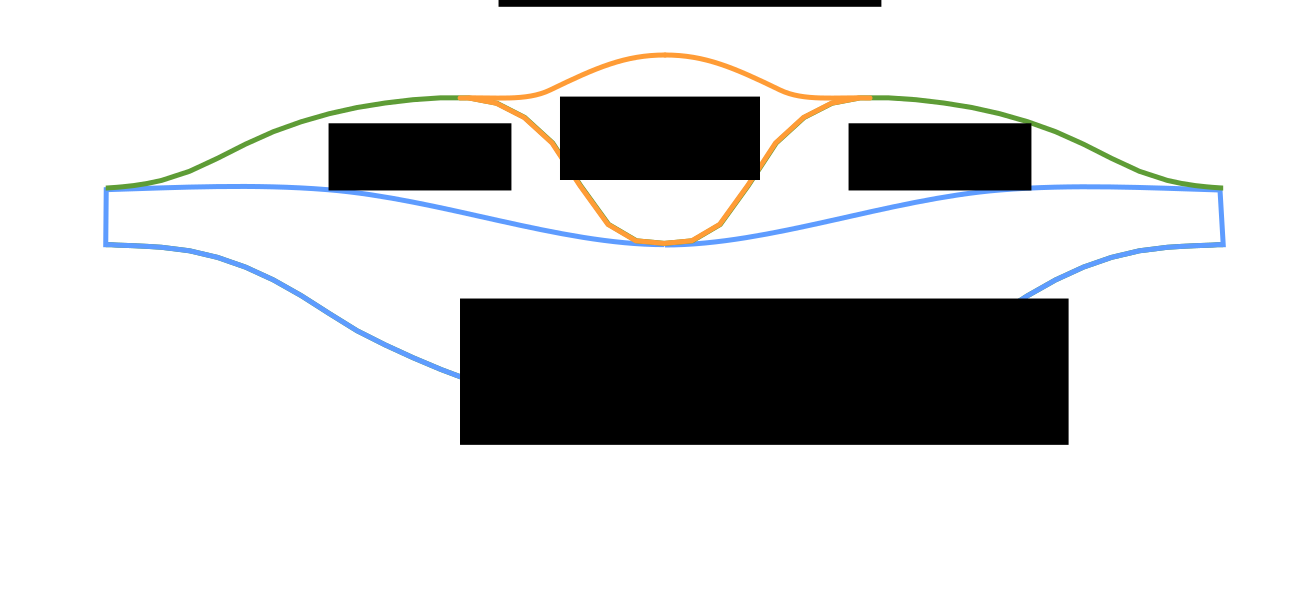
\includegraphics[width=0.8\textwidth]{OriginalSectionWithEngine}
\caption{Вид сечения центроплана в месте стыка передней кромки крыла и фюзеляжа с изображением двигателя}
\label{fig:OriginalSectionWithEngine}
\end{figure}


При такой конфигурации все хорошо (учтены требования малозаметности, аэродинамики).

Но это создает проблему обеспечения прочности центроплана, следовательно проблему весовой эффективности. Наше решение - критическое к созданию конструкции. Если не выйдет, всё летит к черту. Создаем модель по идеальной аэродинамике.

В настоящей работе рассматривается задача проектирования такой конструкции центроплана БПЛА с особенностью, с крылом большого удлинения.

В рамках решения задачи сформирован задел для дальнейшего решения многодисциплинарной задачи по выбору рациональной конфигурации с точки зрения критерия эффективности (по улучшению компоновки) с учетом возможного изменения внешней геометрии.

Описываем: для решения задачи в работе проведено концептуальное исследование зависимости весовых, прочностных и жесткостных характеристик конструкции от геометрических параметров, определяющих форму центроплана.

В работе также рассмотрены и приведены программные средства, предназначенные для решения подобных (параметрических, проектировочных) задач. И даны описания модификаций программы.

В работе сформирована КЭ параметрическая модель и проведены валидационные исследования этой модели. НА ней же проведены весовые оценки. 

 
\chapter{Разработка рациональной конструкции}

\section{Требования и ограничения}


В работе был рассмотрен ?вопрос проектировки? беспилотного летательного аппарата (БПЛА), предназаченного для длительного ($\approx24$~часа без дозаправки) барражирования в целях мониторинга и разведки (ограничения по режимам полета представлены на Рис.\ref{fig:ModeOfFlight}). В связи с этим к БПЛА были предъявлены высокие требования по малозаметности и аэродинамическому качеству. 


За основу была взята разработанная в ЦАГИ модель БПЛА, хорошо отвечающая требованиям аэродинамического качества и малозаметности. Вид фюзеляжа выбранной модели показан на Рис.\ref{fig:BPLA_TSAGI}.
 

%Возможно, вставить пункт с геометрическими ограничениями
  
  



\begin{figure}[ht]
\centering
\includegraphics[width=1\textwidth]{BPS_Catia_Full}
\caption{Вид модели БПЛА-ЦАГИ}
\label{fig:BPLA_TSAGI}
\end{figure}

Данная модель выполнена по схеме ``бесхвостка'' с крылом большого удлинения, интегрированным с фюзеляжем. 

Для интеграции двигателя с воздухозаборником в конструкцию данной модели в конструкции используется изогнутый центроплан. Использование такой формы центроплана сопряжено с возможным возникновением проблем обеспечения прочности в связи с большими изгибающими моментами в нём. 

Использование такого центроплана может существенно ухудшить компоновку и весовую эффективность БПЛА по сравнению с использованием прямого центроплана. Исследований центропланов такой формы ранее не проводилось. В данной работе проведен анализ возможных ухудшений весовой эффективности. 
 
%очевидно, что волнообразный центроплан может иметь напряжные вопросы с обеспечением прочности, т.к. такие центропланы в такой размерности не использовались, довольно нагружены. Сказать про компоновку, нарисовать её (общие вещи).

%с самого начала пишем, какие проблемы. Так сделали, такая компоновка, но у неё такие-то проблемы след волнообразный центроплан

%дальше: это может существенно ухудшить компоновку и весовую эффективность по сравнению с прямым центропланом. Цель работы - оценить возможные ухудшения. 

% и уже для того, чтобы оценить: следующий параграф 

Для оценки возможных ухудшений весовой эффективности и компоновки была поставлена задача построения расчетной модели данного БПЛА и прочностного анализа созданной модели. 
При построении модели необходимо было учесть ее дальнейшую модификацию, позволяющую варьировать форму внешних аэродинамических обводов. В бакалаврской работе форма внешних аэродинамических обводов постоянны. Также постоянными считаются нагрузки на конструкцию (см.Раздел \ref{sec:externalLoads}). 

%В бакалаврской работе будем рассматривать только те обводы, которые есть в этой модели. И целью работы будет оценка потерь из-за такого центроплана (в прочности)

 
  
  

%Не забыть про то, что мы также хотим менять аэродинамику
%Требования: БПЛА, полет на таких-то высотах, столько-то. Весовая сводка такая-то, максимальные перегрузки, коэффициент запаса, аэродинамика. Ограничения - малозаметность, вес, пожаробезопасность отсека двигателя. 
%




\section{Компоновочная схема}
На рисунках 
\ref{fig:BPS_Catia_Top}--\ref{fig:BPS_Catia} показана модель гипотетической конструкции БПЛА.
%\begin{itemize}
%\item размах крыльев: $\approx37\text{м}$
%\item высота фюзеляжа: 1.7м
%\item длина фюзеляжа: 7м
%\end{itemize}


\begin{figure}[H]
\centering
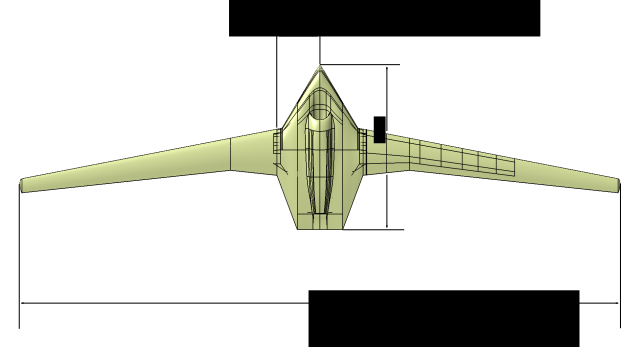
\includegraphics[width=0.8\textwidth]{BPS_Catia_Top}
\caption{Вид сверху}
\label{fig:BPS_Catia_Top}
\end{figure}
%На рисунках проставить размеры

Как видно из рисунков для данной компоновочной схемы используется крыло большого удлинения. Из рисунка \ref{fig:BPS_Catia_WithoutSkin}, на котором представлена базовая конструктивно-силовая схема БПЛА, можно видеть, как происходит интеграция корпуса фюзеляжа, крыла и двигателя. 

\begin{figure}[H]
\centering
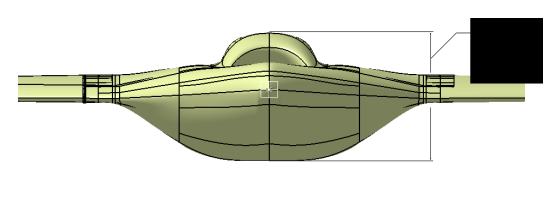
\includegraphics[width=0.8\textwidth]{BPS_Catia_Front}
\caption{Вид фюзеляжа спереди}
\label{fig:BPS_Catia_Front}
\end{figure}




\begin{figure}[H]
\centering
\includegraphics[width=0.8\textwidth]{BPS_Catia}
\caption{Вид фюзеляжа в изометрии}
\label{fig:BPS_Catia}
\end{figure}

%\begin{figure}[H]
%\centering
%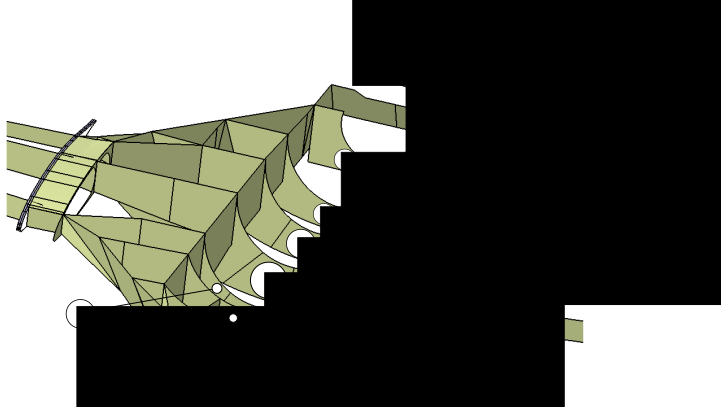
\includegraphics[width=0.8\textwidth]{BPS_Catia_WithoutSkin}
%\caption{Вид фюзеляжа со снятой обшивкой}
%\label{fig:BPS_Catia_WithoutSkin}
%\end{figure}

\begin{figure}[H]
\centering
\def\svgwidth{0.9\textwidth}
\input{figures/BPS_Catia_WithoutSkin.pdf_tex}
\caption{Вид фюзеляжа со снятой обшивкой с указанием узлов крепления шасси и двигателя}
\label{fig:BPS_Catia_WithoutSkin}
\end{figure}

Из рисунка видно, что двигатель с воздухозаборником значительно утоплены и находятся практически в середине фюзеляжа. Как уже отмечалось выше, эта особенность позволяет значительно улучшить малозаметность и аэродинамическое качество самолета (ссылка на отчет), но приводит к необходимости формировать искривленный центроплан. 

Формирование искривленного центроплана создает дополнительные проблемы из-за большой величины изгибающего момента в корне крыла. Еще одной проблемой обеспечения прочности корпуса БПЛА является высокая чувствительность параметров управляемости БПЛА от жесткостных характеристик корпуса и особенно зоны стыка крыла с центропланом, где расположены узлы крепления стоек основного шасси. Очевидно, что для решения проектировочной задачи необходимо проведение комплексных исследований прочности данной конструкции включая анализ прочности, устойчивости и управляемости. 

В данной схеме используется только горизонтальное оперение: руль высоты. Механизация крыла состоит из расщепляющихся элеронов на концах крыльев, элевонов и интерцепторов. В качестве тяги используется один реактивный двигатель, установленный в канале воздухозаборника. Места креплений стоек и замков шасси, расположение двигателя и узлов его крепления показаны на Рис. \ref{fig:BPS_Catia_Top_WithoutSkin}. 


\begin{figure}[H]
\centering
\def\svgwidth{0.9\textwidth}
\input{figures/BPS_Catia_Top_WithoutSkin.pdf_tex}
\caption{Вид сверху без обшивки с указанием узлов крепления шасси и двигателя}
\label{fig:BPS_Catia_Top_WithoutSkin}
\end{figure}

Отсеки фюзеляжа делятся на несколько групп по назначению. Распределение отсеков фюзеляжа по назначению представлено на Рис.\ref{fig:BPS_Catia_Top_PartRoles}. 

На рис.\ref{fig:BPS_Catia_Top_PartRoles} схематически показаны основные отсеки конструкции БПЛА. 

\begin{figure}[H]
\centering
\def\svgwidth{0.9\textwidth}
\input{figures/BPS_Catia_Top_PartRoles.pdf_tex}
\caption{Вид сверху с обозначением роли отсеков}
\label{fig:BPS_Catia_Top_PartRoles}
\end{figure}




%Пока кратко: Крыло большого удлинения интегрировано с фюзеляжем. Двигатель утоплен в конструкцию, подвод воздухозаборника, сопло над горизонтальным оперением. В передней части фюзеляжа расположены отсеки с БРЭО, отсеки с топливом, отсек под переднее шасси. 
% задней части фюзеляжа пара отсеков под топливо, отсеки под БРЭО, шассийные отсеки, шасси крепится на стыке крыла с фюзеляжем. 







%Описываем полностью всю конструкцию. Показываем много разных картинок. 	

\section{Внешние нагрузки}
Основные случаи нагружения. Какой случай нагружения рассматривается (кажется, A', т.е. выход из пикирования), эпюры нагрузок  

\section{Расчетные прочностные модели}
Здесь про 3 КСС пока молчим, расписываем лишь построение модели
%\section{Создание конечно-элементной модели проектируемого самолета}

В ходе работы были исследованы вопросы построения проектировочной модели БПЛА с крылом большого удлинения и несущим фюзеляжем. При помощи программного комплекса ``Conver'' (см. раздел \ref{sec:Conver}), исходя из взятой за основу концептуальной модели, была создана МКЭ-модель проектируемого БПЛА с исключенной верхней частью воздухозаборника, не несущей в себе силовых элементов. 

%\begin{figure}[ht]
%\centering
%\includegraphics[width=0.8\textwidth]{BPLAfullModel}
%\caption{МКЭ-модель проектируемого БПЛА без верхней части}
%\label{fig:BPLAfullModel}
%\end{figure}

\subsection{Требования к прочностной модели}

К прочностной модели предъявляются следующие требования:

\begin{enumerate}
\item оперативность построения модели
\item подробность модели
\item надежность анализа
\item возможность модификации 
\item рациональный выбор конечно-элементной сетки
\end{enumerate}

%Выбор базового комплекса
\subsection{Выбор базового комплекса}
Учитывая представленные выше требования к модели, для построения моделей в работе был использован программный комплекс ``Conver'', разработанный в НИО-3 ЦАГИ. 
% в описании конвера расписывать, чем он нам подходит
%\subsection{Программный комплекс ``Conver''}
\label{sec:Conver}

Для построения описанных выше моделей использовался разработанный в ЦАГИ программный комплекс ``Conver''. Его использование позволило многократно сократить время построения каждой модели. 

%\subsection{Описание комплекса}
Комплекс представляет собой многоуровневую среду для автоматизированного проектирования и оптимизации ЛА. Комплекс делится на 4 уровня по степени детализации:



\begin{figure}[ht]
\centering
\includegraphics[width=0.6\textwidth]{ConverCircle} 
\caption{Принципиальная схема четырехуровневого проектирования}
\end{figure}



\begin{itemize}
\item Уровень 1: расчёт аэродинамических нагрузок и аэродинамических характеристик; 
\item Уровень 2: расчёт инерционных нагрузок, формирование случаев нагружения, решение задач статической и динамической аэроупругости, анализ веса конструкции планера;
\item Уровень 3: расчёт местной и общей устойчивости, анализ закритического состояния отдельных элементов конструкции, расчёт нелинейного НДС панелей гермокабины, расчет несущей способности элементов конструкции;
\item Уровень 4: расчёт общего НДС конструкции ЛА, определение запасов прочности, определение остаточной прочности, расчет длительной прочности.
\end{itemize}

Основные особенности программного комплекса:

\begin{enumerate}
\item Эффективное проведение параметрических исследований для различных конструкций планера, что позволяет минимизировать временные затраты и снизить трудоёмкость всего процесса;
\item Обеспечение более высокого качественного уровня параметрических исследований на начальной стадии проектирования за счёт автоматизированного создания полноразмерных моделей конструкции ЛА и автоматизации процесса анализа результатов исследований;
\item Оперативная оценка веса конструкций летательных аппаратов с учётом технологических ограничений при автоматическом использовании специализированных баз данных поправочных технологических коэффициентов.
\end{enumerate}

%Нарисовать блок-схему взаимодействия nastran patran conver расчетная модель автокад аэродинамика


%\input{sections/reworkingConver}

\subsection{Создание модели}
\label{sec:creationOfOneModel}
\subsubsection{Создание геометрии}
Показать скриншоты из List1,2,4,
\subsubsection{Задание нагрузок и свойств отсеков}
Показать скриншот из ListAdd
\subsubsection{Построение МКЭ-модели}
Показать скриншот из ListA, скрин из патрана. 


%\subsection{Программный комплекс ``Conver''}
\label{sec:Conver}

Для построения описанных выше моделей использовался разработанный в ЦАГИ программный комплекс ``Conver''. Его использование позволило многократно сократить время построения каждой модели. 

%\subsection{Описание комплекса}
Комплекс представляет собой многоуровневую среду для автоматизированного проектирования и оптимизации ЛА. Комплекс делится на 4 уровня по степени детализации:



\begin{figure}[ht]
\centering
\includegraphics[width=0.6\textwidth]{ConverCircle} 
\caption{Принципиальная схема четырехуровневого проектирования}
\end{figure}



\begin{itemize}
\item Уровень 1: расчёт аэродинамических нагрузок и аэродинамических характеристик; 
\item Уровень 2: расчёт инерционных нагрузок, формирование случаев нагружения, решение задач статической и динамической аэроупругости, анализ веса конструкции планера;
\item Уровень 3: расчёт местной и общей устойчивости, анализ закритического состояния отдельных элементов конструкции, расчёт нелинейного НДС панелей гермокабины, расчет несущей способности элементов конструкции;
\item Уровень 4: расчёт общего НДС конструкции ЛА, определение запасов прочности, определение остаточной прочности, расчет длительной прочности.
\end{itemize}

Основные особенности программного комплекса:

\begin{enumerate}
\item Эффективное проведение параметрических исследований для различных конструкций планера, что позволяет минимизировать временные затраты и снизить трудоёмкость всего процесса;
\item Обеспечение более высокого качественного уровня параметрических исследований на начальной стадии проектирования за счёт автоматизированного создания полноразмерных моделей конструкции ЛА и автоматизации процесса анализа результатов исследований;
\item Оперативная оценка веса конструкций летательных аппаратов с учётом технологических ограничений при автоматическом использовании специализированных баз данных поправочных технологических коэффициентов.
\end{enumerate}

%Нарисовать блок-схему взаимодействия nastran patran conver расчетная модель автокад аэродинамика


%\section{Программный комплекс ``Conver''}

\subsection{Описание комплекса}
Комплекс представляет собой многоуровневую среду для автоматизированного проектирования и оптимизации ЛА. Комплекс делится на 4 уровня по степени детализации:



\begin{figure}[ht]
\centering
\includegraphics[width=0.6\textwidth]{ConverCircle} 
\caption{Принципиальная схема четырехуровневого проектирования}
\end{figure}



\begin{itemize}
\item Уровень 1: расчёт аэродинамических нагрузок и аэродинамических характеристик; 
\item Уровень 2: расчёт инерционных нагрузок, формирование случаев нагружения, решение задач статической и динамической аэроупругости, анализ веса конструкции планера;
\item Уровень 3: расчёт местной и общей устойчивости, анализ закритического состояния отдельных элементов конструкции, расчёт нелинейного НДС панелей гермокабины, расчет несущей способности элементов конструкции;
\item Уровень 4: расчёт общего НДС конструкции ЛА, определение запасов прочности, определение остаточной прочности, расчет длительной прочности.
\end{itemize}

Основные особенности программного комплекса:

\begin{enumerate}
\item Эффективное проведение параметрических исследований для различных конструкций планера, что позволяет минимизировать временные затраты и снизить трудоёмкость всего процесса;
\item Обеспечение более высокого качественного уровня параметрических исследований на начальной стадии проектирования за счёт автоматизированного создания полноразмерных моделей конструкции ЛА и автоматизации процесса анализа результатов исследований;
\item Оперативная оценка веса конструкций летательных аппаратов с учётом технологических ограничений при автоматическом использовании специализированных баз данных поправочных технологических коэффициентов.
\end{enumerate}


\subsection{Внесенные изменения}

В ходе работы был создан новый интерфейс  для первого уровня комплекса. 

\begin{figure}[h]
\centering
\includegraphics[width=0.8\textwidth]{ConverNewInterfaceOverview}
\caption{Новый интерфейс программного комплекса ``Conver''}
\label{fig:ConverNewInterfaceOverview}
\end{figure}


В новом интерфейсе были реализованы следующие изменения:

\begin{itemize}
	\item Полностью переработана система визуализации
	\begin{itemize}
		\item Добавлены инструменты масштаба и перемещения
		\item Добавлена двусторонняя связь между схемой и областями ввода данных
		\item Добавлена возможность отображения каждого этажа в 		схеме по отдельности
		\item Добавлено отображение ошибок во введенных данных
	\end{itemize}
	\item Переработана система ввода параметров отсеков
	\begin{itemize}
		\item Добавлены визуальные подсказки, предупреждающие ошибки в данных
		\item Добавлена возможность ввода параметров сразу для нескольких отсеков
	\end{itemize}
	\item Добавлена возможность ввода нагрузок непосредственно через задание сил, действующих на отсек
	\item Добавлена возможность просмотра данных, получаемых из других уровней комплекса:
	\begin{itemize}
		\item Оценочный расчет веса конструкции или выбранных отсеков
		\item Расчет объема выбранных отсеков
		\item Просмотр площадей стенок отсеков
	\end{itemize}
\end{itemize}

Рассмотрим, как изменилась работа с типовыми операциями, с которыми приходится сталкиваться пользователю. 


\subsection{Сравнение работы с типовыми операциями в старой и новой версии интерфейса}

\subsubsection{Изменение толщин в отсеке}

Задача: изменить толщину отсека в центроплане. 

\paragraph{Прежний подход:} 

\begin{itemize}
\item Найти номер отсека по схеме (Рис.\ref{fig:ConverListxzOld}) ($\sim1-3~\text{мин.}$)
\item Найти соответствующую ячейку в таблице толщин. ($\sim15~\text{сек.}$)
\item Изменить значение в ячейке. ($\sim5~\text{сек.}$)
\end{itemize}

Итого: $\sim3~\text{мин.}$

\begin{figure}[ht]
\centering
\includegraphics[width=0.8\textwidth]{ConverListxzOld}
\caption{Окно отображения отсеков в предыдущей версии интерфейса}
\label{fig:ConverListxzOld}
\end{figure}

\paragraph{Новый подход:}

\begin{itemize}
\item Кликнуть на нужный отсек на схеме (Рис.\ref($\sim5~\text{сек.}$)
\item Изменить значение в ячейке толщины нужной стенки($\sim5~\text{сек.}$)
\end{itemize}

Итого: $\sim10~\text{сек.}$

\begin{figure}[ht]
\centering
\includegraphics[width=0.8\textwidth]{ConverNewChangingThicks}
\caption{Окно отображения отсеков в новой версии интерфейса}
\label{ConverNewChangingThicks}
\end{figure}

\subsubsection{Нагружение отсека заданной силой}

Задача: по визуальному нахождению стенки нагрузить её заданной силой.

\paragraph{Прежний подход:}

\begin{itemize}
\item Найти по схеме (Рис.\ref{fig:ConverListxzOld}) отсеки, в которых может быть определена нужная стенка ($\sim5~\text{мин.}$)
\item Найти в таблице толщин, какой из выбранных отсеков имеет толщину этой стенки отличную от нуля($\sim3~\text{мин.}$)
\item Из 4 уровня программы найти площадь этой стенки($\sim3~\text{мин.}$)
\item По площади стенки найти давление, которое необходимо на неё приложить($\sim1~\text{мин.}$)
\item В таблице давлений найти нужную ячейку и ввести в неё полученную величину($\sim5~\text{мин.}$)
\end{itemize}

Итого: $\sim17~\text{мин.}$

\paragraph{Новый подход:}

\begin{itemize}
\item Кликнуть на один из отсеков, которому принадлежит эта стенка($\sim10~\text{сек.}$)
\item Если ячейка давления на нужную стенку выделена красным, выбрать другой отсек, в котором эта ячейка не выделена красным, то есть в которой эта стенка имеет ненулевую толщину($\sim1~\text{мин.}$)
\item Нажать кнопку ``Add load''  ($\sim10~\text{сек.}$)
\item В открывшемся окне (Рис.\ref{fig:ConverAddLoad}) ввести величину прикладываемой силы и выбрать стенки отсека, на которые должна быть распределена данная нагрузка. ($\sim30~\text{сек.}$) 
\item Нажать ``Add load'' ($\sim10~\text{сек.}$)

\end{itemize}

Итого: $\sim2~\text{мин.}$

\begin{figure}[ht]
\centering
\includegraphics[width=0.5\textwidth]{ConverNewInterfaceAddLoad}
\caption{Окно добавления нагрузок в новой версии интерфейса}
\label{fig:ConverAddLoad}
\end{figure}


\section{Особенности НДС}
Корень крыла, штаны
%\subsection{Проблемы проектирования}


Обшивка почти не нагружена, можно использовать композиты. Наибольшие напряжения в центроплане - необходим достаточно жесткий короб. Отдельно нужно рассмотреть штаны (на устойчивость рассмотрим сейчас, варианты исполнения в третьей главе) 

В корне крыла Q=13,7тс, Мизг=80 тс*м
На изломе крыла Q=10,3тс, Мизг=55 тс*м

%В предложенной конструкторами схеме были выявлены некоторые проблемные места, в которых требовался дополнительный анализ. 


\begin{figure}[H]
\centering
\def\svgwidth{0.9\textwidth}
\input{figures/WingDeformation.pdf_tex}
\caption{Эпюра перемещений задней кромки крыла}
\label{fig:WingDeformation}
\end{figure}

 \subsection{Крепление хвостовой части к кессону центроплана} 
\label{sec:pants}
\begin{figure}[H]
\centering
\includegraphics[width=0.6\textwidth]{IsoviewOfPantsBW}
\caption{Вид центральной части фюзеляжа с выделенными стенками}
\label{fig:IsoviewOfPants}
\end{figure}

Для предварительной оценки НДС наиболее нагруженных деталей и узлов хвостовой части корпуса БПЛА была решена модельная задача по оценке нагруженности вертикальных стенок, обеспечивающих передачу нагрузок от двигателя, оборудования и топлива на конструкцию центроплана (стенки обозначены на Рис.~\ref{fig:IsoviewOfPants} серой заливкой, светло-серой заливкой обозначены зоны основных узлов крепления двигателя). Уровень нагружения был оценен на основе аналитических формул. Схема нагружения модельных стенок показана на Рис.\ref{fig:IsoviewOfPantsModel}.

\begin{figure}[H]
\centering
%\def\svgwidth{0.9\textwidth}
\input{figures/IsoviewOfPantsModel.pdf_tex}
\caption{Схема нагружения модельных стенок}
\label{fig:IsoviewOfPantsModel}
\end{figure}

%
%\begin{figure}[H]
%\centering
%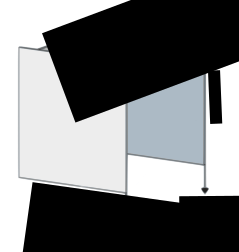
\includegraphics[width=0.8\textwidth]{IsoviewOfPantsModel}
%\caption{Схема нагружения модельных стенок}
%\label{IsoviewOfPantsModel}
%\end{figure}


Уровень нагружения оценивался по величинам касательных напряжений. Касательные напряжения в пластине при чистом сдвиге равны

\begin{equation}
\tau=\frac{3}{2}\cdot\frac{Q}{bh}
\end{equation}
Критические по устойчивости касательные напряжения в пластине при чистом сдвиге равны \cite{Volmir}:

\begin{equation}
\tau_\text{кр}=\frac{K}{12}\frac{\pi^2D}{b^2h} = \frac{K}{12}\frac{\pi^2E}{(1-\mu^2)}\left(\frac{h}{b}\right)^2,\, K=5.34 + 4\frac{a}{b},
\end{equation}
где $a$ - размер пластины вдоль направления действия силы, $b$ - размер пластины поперек направления действия силы, $h$ - толщина пластины, $D$ - изгибная жесткость пластины, $E$ - модуль Юнга, $\mu$ - модуль Пуассона материала пластины, $Q$ - приложенная сила.
Допускаемые толщины найдем из условия

\begin{equation}
\tau_\text{кр} \geq \tau \to h \geq \sqrt[3]{\frac{3\cdot12}{2}\frac{Qb\cdot(1-\mu^2)}{k\pi^2E}} 
\end{equation}
Подставляя значения, получим:

\begin{equation}
Q=\frac{8000}{n}\text{кгс},\,a=1300\text{мм},\,b=1009\text{мм},\,\mu=0.3,\,E=7000\frac{\text{кгс}}{\text{мм}^2}
\end{equation}

\begin{equation}
h \geq \sqrt[3]{\frac{18\cdot8000\cdot1000\cdot(1-\mu^2)}{k\pi^2En}} = \frac{5.67}{\sqrt[3]{n}} 
\end{equation}

Таким образом, для случаев $n = 2$ и $n = 4$  были получены минимальные допустимые толщины, 
равные

\begin{equation}
h\geq4.50\text{мм},\,n=2
\end{equation}
\begin{equation}
h\geq2.83\text{мм},\,n=4
\end{equation}
%\subsubsection{Фюзеляжная часть центроплана}

Другим проблемным местом была фюзеляжная часть центроплана. Из-за требований компоновки, а именно интеграции двигателя, центроплан необходимо делать изогнутым (Рис.\ref{fig:centroplan}). Это вносит дополнительные трудности в виде увеличения веса по сравнению с прямым центропланом. Исследованию фюзеляжной части центроплана (выделена серым на Рис.\ref{fig:centroplan}) посвящена глава \ref{chap:SolvingModel}.

\begin{figure}[ht]
\centering
\includegraphics[width=0.6\textwidth]{centroplan}
\caption{Изогнутый центроплан с выделением исследуемой части}
\label{fig:centroplan}
\end{figure}


\section{Рациональные параметры КСС}
Здесь возникает вопрос о разных КСС. Говорим, что сейчас всё решить не сможем, но задел сделаем

Из этого получаем 2 модельные задачи: Кессон и альтернативные КСС. О них в следующих главах.
%\chapter{Проектировочное исследование}
%\section{Создание конечно-элементной модели проектируемого самолета}

В ходе работы были исследованы вопросы построения проектировочной модели БПЛА с крылом большого удлинения и несущим фюзеляжем. При помощи программного комплекса ``Conver'' (см. раздел \ref{sec:Conver}), исходя из взятой за основу концептуальной модели, была создана МКЭ-модель проектируемого БПЛА с исключенной верхней частью воздухозаборника, не несущей в себе силовых элементов. 

%\begin{figure}[ht]
%\centering
%\includegraphics[width=0.8\textwidth]{BPLAfullModel}
%\caption{МКЭ-модель проектируемого БПЛА без верхней части}
%\label{fig:BPLAfullModel}
%\end{figure}

\subsection{Требования к прочностной модели}

К прочностной модели предъявляются следующие требования:

\begin{enumerate}
\item оперативность построения модели
\item подробность модели
\item надежность анализа
\item возможность модификации 
\item рациональный выбор конечно-элементной сетки
\end{enumerate}

%Выбор базового комплекса
\subsection{Выбор базового комплекса}
Учитывая представленные выше требования к модели, для построения моделей в работе был использован программный комплекс ``Conver'', разработанный в НИО-3 ЦАГИ. 
% в описании конвера расписывать, чем он нам подходит
%\subsection{Программный комплекс ``Conver''}
\label{sec:Conver}

Для построения описанных выше моделей использовался разработанный в ЦАГИ программный комплекс ``Conver''. Его использование позволило многократно сократить время построения каждой модели. 

%\subsection{Описание комплекса}
Комплекс представляет собой многоуровневую среду для автоматизированного проектирования и оптимизации ЛА. Комплекс делится на 4 уровня по степени детализации:



\begin{figure}[ht]
\centering
\includegraphics[width=0.6\textwidth]{ConverCircle} 
\caption{Принципиальная схема четырехуровневого проектирования}
\end{figure}



\begin{itemize}
\item Уровень 1: расчёт аэродинамических нагрузок и аэродинамических характеристик; 
\item Уровень 2: расчёт инерционных нагрузок, формирование случаев нагружения, решение задач статической и динамической аэроупругости, анализ веса конструкции планера;
\item Уровень 3: расчёт местной и общей устойчивости, анализ закритического состояния отдельных элементов конструкции, расчёт нелинейного НДС панелей гермокабины, расчет несущей способности элементов конструкции;
\item Уровень 4: расчёт общего НДС конструкции ЛА, определение запасов прочности, определение остаточной прочности, расчет длительной прочности.
\end{itemize}

Основные особенности программного комплекса:

\begin{enumerate}
\item Эффективное проведение параметрических исследований для различных конструкций планера, что позволяет минимизировать временные затраты и снизить трудоёмкость всего процесса;
\item Обеспечение более высокого качественного уровня параметрических исследований на начальной стадии проектирования за счёт автоматизированного создания полноразмерных моделей конструкции ЛА и автоматизации процесса анализа результатов исследований;
\item Оперативная оценка веса конструкций летательных аппаратов с учётом технологических ограничений при автоматическом использовании специализированных баз данных поправочных технологических коэффициентов.
\end{enumerate}

%Нарисовать блок-схему взаимодействия nastran patran conver расчетная модель автокад аэродинамика


%\input{sections/reworkingConver}

\subsection{Создание модели}
\label{sec:creationOfOneModel}
\subsubsection{Создание геометрии}
Показать скриншоты из List1,2,4,
\subsubsection{Задание нагрузок и свойств отсеков}
Показать скриншот из ListAdd
\subsubsection{Построение МКЭ-модели}
Показать скриншот из ListA, скрин из патрана. 


%\subsection{Проблемы проектирования}


Обшивка почти не нагружена, можно использовать композиты. Наибольшие напряжения в центроплане - необходим достаточно жесткий короб. Отдельно нужно рассмотреть штаны (на устойчивость рассмотрим сейчас, варианты исполнения в третьей главе) 

В корне крыла Q=13,7тс, Мизг=80 тс*м
На изломе крыла Q=10,3тс, Мизг=55 тс*м

%В предложенной конструкторами схеме были выявлены некоторые проблемные места, в которых требовался дополнительный анализ. 


\begin{figure}[H]
\centering
\def\svgwidth{0.9\textwidth}
\input{figures/WingDeformation.pdf_tex}
\caption{Эпюра перемещений задней кромки крыла}
\label{fig:WingDeformation}
\end{figure}

 \subsection{Крепление хвостовой части к кессону центроплана} 
\label{sec:pants}
\begin{figure}[H]
\centering
\includegraphics[width=0.6\textwidth]{IsoviewOfPantsBW}
\caption{Вид центральной части фюзеляжа с выделенными стенками}
\label{fig:IsoviewOfPants}
\end{figure}

Для предварительной оценки НДС наиболее нагруженных деталей и узлов хвостовой части корпуса БПЛА была решена модельная задача по оценке нагруженности вертикальных стенок, обеспечивающих передачу нагрузок от двигателя, оборудования и топлива на конструкцию центроплана (стенки обозначены на Рис.~\ref{fig:IsoviewOfPants} серой заливкой, светло-серой заливкой обозначены зоны основных узлов крепления двигателя). Уровень нагружения был оценен на основе аналитических формул. Схема нагружения модельных стенок показана на Рис.\ref{fig:IsoviewOfPantsModel}.

\begin{figure}[H]
\centering
%\def\svgwidth{0.9\textwidth}
\input{figures/IsoviewOfPantsModel.pdf_tex}
\caption{Схема нагружения модельных стенок}
\label{fig:IsoviewOfPantsModel}
\end{figure}

%
%\begin{figure}[H]
%\centering
%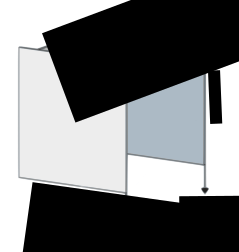
\includegraphics[width=0.8\textwidth]{IsoviewOfPantsModel}
%\caption{Схема нагружения модельных стенок}
%\label{IsoviewOfPantsModel}
%\end{figure}


Уровень нагружения оценивался по величинам касательных напряжений. Касательные напряжения в пластине при чистом сдвиге равны

\begin{equation}
\tau=\frac{3}{2}\cdot\frac{Q}{bh}
\end{equation}
Критические по устойчивости касательные напряжения в пластине при чистом сдвиге равны \cite{Volmir}:

\begin{equation}
\tau_\text{кр}=\frac{K}{12}\frac{\pi^2D}{b^2h} = \frac{K}{12}\frac{\pi^2E}{(1-\mu^2)}\left(\frac{h}{b}\right)^2,\, K=5.34 + 4\frac{a}{b},
\end{equation}
где $a$ - размер пластины вдоль направления действия силы, $b$ - размер пластины поперек направления действия силы, $h$ - толщина пластины, $D$ - изгибная жесткость пластины, $E$ - модуль Юнга, $\mu$ - модуль Пуассона материала пластины, $Q$ - приложенная сила.
Допускаемые толщины найдем из условия

\begin{equation}
\tau_\text{кр} \geq \tau \to h \geq \sqrt[3]{\frac{3\cdot12}{2}\frac{Qb\cdot(1-\mu^2)}{k\pi^2E}} 
\end{equation}
Подставляя значения, получим:

\begin{equation}
Q=\frac{8000}{n}\text{кгс},\,a=1300\text{мм},\,b=1009\text{мм},\,\mu=0.3,\,E=7000\frac{\text{кгс}}{\text{мм}^2}
\end{equation}

\begin{equation}
h \geq \sqrt[3]{\frac{18\cdot8000\cdot1000\cdot(1-\mu^2)}{k\pi^2En}} = \frac{5.67}{\sqrt[3]{n}} 
\end{equation}

Таким образом, для случаев $n = 2$ и $n = 4$  были получены минимальные допустимые толщины, 
равные

\begin{equation}
h\geq4.50\text{мм},\,n=2
\end{equation}
\begin{equation}
h\geq2.83\text{мм},\,n=4
\end{equation}
%\subsubsection{Фюзеляжная часть центроплана}

Другим проблемным местом была фюзеляжная часть центроплана. Из-за требований компоновки, а именно интеграции двигателя, центроплан необходимо делать изогнутым (Рис.\ref{fig:centroplan}). Это вносит дополнительные трудности в виде увеличения веса по сравнению с прямым центропланом. Исследованию фюзеляжной части центроплана (выделена серым на Рис.\ref{fig:centroplan}) посвящена глава \ref{chap:SolvingModel}.

\begin{figure}[ht]
\centering
\includegraphics[width=0.6\textwidth]{centroplan}
\caption{Изогнутый центроплан с выделением исследуемой части}
\label{fig:centroplan}
\end{figure}


%\chapter{Решение модельной задачи}
\label{chap:SolvingModel}

\section{Создание параметрической модели центроплана}
\label{sec:creationOfModel}

В рамках решения задачи была создана упрощенная параметрическая модель центроплана с двумя варьируемыми  параметрами. В упрощенной модели кессон фюзеляжной части центроплана заменен коробом переменного прямоугольного сечения с поперечными стенками. На короб передаются усилия путем приложения аэродинамических нагрузок на упрощенную модель крыла -- короб постоянного прямоугольного сечения (Рис.\ref{fig:CurvedKessonPatran}). Все панели и стенки считаются алюминиевыми, панели и стенки имеют постоянную толщину по их площади, панели и стенки без вырезов. Носовая и хвостовая части самолёта опущены для простоты расчета.  



\begin{figure}[ht]
\centering
\includegraphics[width=0.9\textwidth]{simplifiedCentroplan}
\caption{Упрощенная модель центроплана с выделением исследуемой части}
\label{fig:CurvedKessonPatran}
\end{figure}

Использование в МКЭ-расчете такой упрощенной модели позволяет значительно ускорить процесс прочностного параметрического анализа при тех же вычислительных мощностях. Так, в упрощенной модели используется $\approx10000$ конечных элементов, в то время как в полной модели самолета используется $\approx270000$ конечных элементов.

Как было сказано выше, рассматриваемая модель имеет два варьируемых параметра: относительная координата нижней точки сечения и строительная высота сечения в плоскости XY в плоскости симметрии самолета. В качестве кривых, описывающих нижнюю и верхнюю поверхность кессона выбраны кубические сплайны, построенные через найденные исходя из выбранных параметров точки. Производные сплайнов в точках стыка фюзеляжа с крылом ($z=2.45\text{м}$) и в плоскости симметрии самолета ($z=0\text{м}$) приняты равными нулю. Пример модельного сечения центроплана в плоскости YZ приведен на Рис.\ref{fig:KessSectionExample}.

\begin{figure}[ht]
\centering
%\def\svgwidth{1\textwidth}
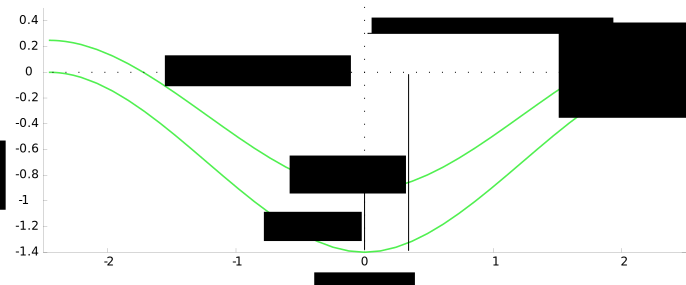
\includegraphics[width=1\textwidth]{KessSectionExample}
%\input{figures/KessSectionExample.pdf_tex}
\caption{Пример модельного поперечного сечения центроплана}
\label{fig:KessSectionExample}
\end{figure}


Выбор такой параметрической модели позволит в дальнейшем (вне рамок данной работы) включить в процесс оптимизации сечения также расчет аэродинамических нагрузок, что позволит полностью автоматизировать процесс оптимизации формы центроплана для центропланов такого типа. 


\section{Программный комплекс ``Conver''}

\subsection{Описание комплекса}
Комплекс представляет собой многоуровневую среду для автоматизированного проектирования и оптимизации ЛА. Комплекс делится на 4 уровня по степени детализации:



\begin{figure}[ht]
\centering
\includegraphics[width=0.6\textwidth]{ConverCircle} 
\caption{Принципиальная схема четырехуровневого проектирования}
\end{figure}



\begin{itemize}
\item Уровень 1: расчёт аэродинамических нагрузок и аэродинамических характеристик; 
\item Уровень 2: расчёт инерционных нагрузок, формирование случаев нагружения, решение задач статической и динамической аэроупругости, анализ веса конструкции планера;
\item Уровень 3: расчёт местной и общей устойчивости, анализ закритического состояния отдельных элементов конструкции, расчёт нелинейного НДС панелей гермокабины, расчет несущей способности элементов конструкции;
\item Уровень 4: расчёт общего НДС конструкции ЛА, определение запасов прочности, определение остаточной прочности, расчет длительной прочности.
\end{itemize}

Основные особенности программного комплекса:

\begin{enumerate}
\item Эффективное проведение параметрических исследований для различных конструкций планера, что позволяет минимизировать временные затраты и снизить трудоёмкость всего процесса;
\item Обеспечение более высокого качественного уровня параметрических исследований на начальной стадии проектирования за счёт автоматизированного создания полноразмерных моделей конструкции ЛА и автоматизации процесса анализа результатов исследований;
\item Оперативная оценка веса конструкций летательных аппаратов с учётом технологических ограничений при автоматическом использовании специализированных баз данных поправочных технологических коэффициентов.
\end{enumerate}


\subsection{Внесенные изменения}

В ходе работы был создан новый интерфейс  для первого уровня комплекса. 

\begin{figure}[h]
\centering
\includegraphics[width=0.8\textwidth]{ConverNewInterfaceOverview}
\caption{Новый интерфейс программного комплекса ``Conver''}
\label{fig:ConverNewInterfaceOverview}
\end{figure}


В новом интерфейсе были реализованы следующие изменения:

\begin{itemize}
	\item Полностью переработана система визуализации
	\begin{itemize}
		\item Добавлены инструменты масштаба и перемещения
		\item Добавлена двусторонняя связь между схемой и областями ввода данных
		\item Добавлена возможность отображения каждого этажа в 		схеме по отдельности
		\item Добавлено отображение ошибок во введенных данных
	\end{itemize}
	\item Переработана система ввода параметров отсеков
	\begin{itemize}
		\item Добавлены визуальные подсказки, предупреждающие ошибки в данных
		\item Добавлена возможность ввода параметров сразу для нескольких отсеков
	\end{itemize}
	\item Добавлена возможность ввода нагрузок непосредственно через задание сил, действующих на отсек
	\item Добавлена возможность просмотра данных, получаемых из других уровней комплекса:
	\begin{itemize}
		\item Оценочный расчет веса конструкции или выбранных отсеков
		\item Расчет объема выбранных отсеков
		\item Просмотр площадей стенок отсеков
	\end{itemize}
\end{itemize}

Рассмотрим, как изменилась работа с типовыми операциями, с которыми приходится сталкиваться пользователю. 


\subsection{Сравнение работы с типовыми операциями в старой и новой версии интерфейса}

\subsubsection{Изменение толщин в отсеке}

Задача: изменить толщину отсека в центроплане. 

\paragraph{Прежний подход:} 

\begin{itemize}
\item Найти номер отсека по схеме (Рис.\ref{fig:ConverListxzOld}) ($\sim1-3~\text{мин.}$)
\item Найти соответствующую ячейку в таблице толщин. ($\sim15~\text{сек.}$)
\item Изменить значение в ячейке. ($\sim5~\text{сек.}$)
\end{itemize}

Итого: $\sim3~\text{мин.}$

\begin{figure}[ht]
\centering
\includegraphics[width=0.8\textwidth]{ConverListxzOld}
\caption{Окно отображения отсеков в предыдущей версии интерфейса}
\label{fig:ConverListxzOld}
\end{figure}

\paragraph{Новый подход:}

\begin{itemize}
\item Кликнуть на нужный отсек на схеме (Рис.\ref($\sim5~\text{сек.}$)
\item Изменить значение в ячейке толщины нужной стенки($\sim5~\text{сек.}$)
\end{itemize}

Итого: $\sim10~\text{сек.}$

\begin{figure}[ht]
\centering
\includegraphics[width=0.8\textwidth]{ConverNewChangingThicks}
\caption{Окно отображения отсеков в новой версии интерфейса}
\label{ConverNewChangingThicks}
\end{figure}

\subsubsection{Нагружение отсека заданной силой}

Задача: по визуальному нахождению стенки нагрузить её заданной силой.

\paragraph{Прежний подход:}

\begin{itemize}
\item Найти по схеме (Рис.\ref{fig:ConverListxzOld}) отсеки, в которых может быть определена нужная стенка ($\sim5~\text{мин.}$)
\item Найти в таблице толщин, какой из выбранных отсеков имеет толщину этой стенки отличную от нуля($\sim3~\text{мин.}$)
\item Из 4 уровня программы найти площадь этой стенки($\sim3~\text{мин.}$)
\item По площади стенки найти давление, которое необходимо на неё приложить($\sim1~\text{мин.}$)
\item В таблице давлений найти нужную ячейку и ввести в неё полученную величину($\sim5~\text{мин.}$)
\end{itemize}

Итого: $\sim17~\text{мин.}$

\paragraph{Новый подход:}

\begin{itemize}
\item Кликнуть на один из отсеков, которому принадлежит эта стенка($\sim10~\text{сек.}$)
\item Если ячейка давления на нужную стенку выделена красным, выбрать другой отсек, в котором эта ячейка не выделена красным, то есть в которой эта стенка имеет ненулевую толщину($\sim1~\text{мин.}$)
\item Нажать кнопку ``Add load''  ($\sim10~\text{сек.}$)
\item В открывшемся окне (Рис.\ref{fig:ConverAddLoad}) ввести величину прикладываемой силы и выбрать стенки отсека, на которые должна быть распределена данная нагрузка. ($\sim30~\text{сек.}$) 
\item Нажать ``Add load'' ($\sim10~\text{сек.}$)

\end{itemize}

Итого: $\sim2~\text{мин.}$

\begin{figure}[ht]
\centering
\includegraphics[width=0.5\textwidth]{ConverNewInterfaceAddLoad}
\caption{Окно добавления нагрузок в новой версии интерфейса}
\label{fig:ConverAddLoad}
\end{figure}
\section{Расчет параметрической модели}

Для проведения расчета были выбраны 42 пары значений параметров. Для каждой пары была проведена оптимизация толщин панелей кессона с целью удовлетворения требованиям прочности конструкции, а именно: среднее напряжение в каждой панели не должно превышать значения допускаемого напряжения, принятого равным $35\text{кг}/\text{мм}^2$. Оптимизация проводилась путем вычисления запаса прочности для каждой пластины с последующим делением толщины панели на полученное значение (так называемый алгоритм $\sigma/\sigma$). Итоговые результаты вычислений приведены в таблицах \ref{tab:KessOptimBigTable}, \ref{tab:KessOptimBigTableNormed} и на Рис.\ref{fig:Optimization3dplot} (серым цветом на изображениях сечений показано оригинальное сечение кессона, зеленым - сечение в параметрической модели)  

\tabulinesep = 1mm
\definecolor{lightgray}{gray}{0.9}
\begin{table}[H]
\captionsetup{justification=centering}
\caption{Зависимость площади панелей центроплана и веса кессона от параметров центроплана}
%\rowcolors{2}{}{lightgray}
\begin{tabu}to \linewidth{|c|*4{X[m c]|}*4{X[m c]|}}
\hline
\multirow{2}{*}[-1.1ex]{N} & \multicolumn{4}{c|}{Вес кессона~[кг]} & \multicolumn{4}{c|}{Площадь панелей центроплана~[$\text{м}^2$]} \\ \cline{2-9}
& Верхние панели & Нижние панели & Боковые стенки & $\Sigma$ & Верхние панели & Нижние панели & Боковые стенки & $\Sigma$ \\
\hline
\taburowcolors {lightgray .. white}
0.000  & 0.249 & 297.182 & 294.551 & 12.561 & 604.294 & 2.730 & 2.730 & 4.000 & 9.520\\ \hline
0.000  & 0.403 & 225.261 & 237.378 & 27.672 & 490.313 & 2.730 & 2.740 & 5.210 & 10.720\\ \hline
0.000  & 0.481 & 190.080 & 222.327 & 49.159 & 461.564 & 2.730 & 2.760 & 5.820 & 11.340\\ \hline
0.000  & 0.558 & 161.544 & 211.467 & 65.963 & 438.972 & 2.730 & 2.760 & 6.450 & 11.950\\ \hline
0.000  & 0.635 & 146.581 & 199.989 & 66.844 & 413.415 & 2.730 & 2.780 & 7.090 & 12.590\\ \hline
0.000  & 0.712 & 134.746 & 191.293 & 70.912 & 396.952 & 2.730 & 2.800 & 7.640 & 13.200\\ \hline
-0.800 & 0.249 & 350.816 & 374.021 & 47.679 & 772.515 & 2.910 & 2.910 & 4.000 & 9.850\\ \hline
-0.800 & 0.403 & 253.752 & 259.311 & 53.180 & 566.245 & 2.910 & 2.850 & 5.210 & 10.990\\ \hline
-0.800 & 0.481 & 213.881 & 226.655 & 57.618 & 498.154 & 2.910 & 2.830 & 5.840 & 11.570\\ \hline
-0.800 & 0.558 & 188.442 & 205.603 & 62.047 & 456.092 & 2.910 & 2.810 & 6.450 & 12.150\\ \hline
-0.800 & 0.635 & 174.466 & 196.192 & 66.506 & 437.164 & 2.910 & 2.780 & 7.090 & 12.770\\ \hline
-0.800 & 0.712 & 154.328 & 195.919 & 70.963 & 421.210 & 2.910 & 2.770 & 7.680 & 13.350\\ \hline
-1.000 & 0.249 & 363.681 & 391.414 & 48.862 & 803.953 & 3.010 & 3.000 & 4.000 & 10.000\\ \hline
-1.000 & 0.403 & 258.118 & 275.555 & 53.209 & 586.883 & 3.010 & 2.930 & 5.230 & 11.160\\ \hline
-1.000 & 0.481 & 225.322 & 238.220 & 57.604 & 521.145 & 3.010 & 2.890 & 5.820 & 11.720\\ \hline
-1.000 & 0.558 & 201.612 & 214.755 & 62.046 & 478.413 & 3.010 & 2.860 & 6.440 & 12.310\\ \hline
-1.000 & 0.635 & 171.877 & 203.370 & 66.418 & 441.665 & 3.010 & 2.840 & 7.050 & 12.900\\ \hline
-1.000 & 0.712 & 163.553 & 201.207 & 70.912 & 435.673 & 3.010 & 2.820 & 7.660 & 13.480\\ \hline
-1.100 & 0.249 & 380.079 & 398.521 & 49.032 & 827.631 & 3.050 & 3.050 & 4.000 & 10.110\\ \hline
-1.100 & 0.403 & 267.143 & 279.590 & 53.134 & 599.866 & 3.050 & 2.980 & 5.210 & 11.240\\ \hline
-1.100 & 0.481 & 231.158 & 238.954 & 57.667 & 527.779 & 3.050 & 2.930 & 5.820 & 11.820\\ \hline
-1.100 & 0.558 & 197.327 & 218.001 & 62.040 & 477.368 & 3.050 & 2.910 & 6.410 & 12.390\\ \hline
-1.100 & 0.635 & 191.553 & 205.935 & 66.481 & 463.971 & 3.050 & 2.870 & 7.070 & 12.980\\ \hline
-1.100 & 0.712 & 158.352 & 203.948 & 70.897 & 433.199 & 3.050 & 2.850 & 7.660 & 13.560\\ \hline
-1.200 & 0.249 & 383.525 & 410.374 & 50.351 & 844.249 & 3.110 & 3.110 & 4.000 & 10.210\\ \hline
-1.200 & 0.403 & 279.228 & 288.331 & 53.186 & 620.745 & 3.110 & 3.030 & 5.210 & 11.350\\ \hline
-1.200 & 0.481 & 233.614 & 249.500 & 57.583 & 540.696 & 3.110 & 2.990 & 5.820 & 11.910\\ \hline
-1.200 & 0.558 & 213.922 & 221.683 & 62.125 & 497.728 & 3.110 & 2.950 & 6.450 & 12.500\\ \hline
-1.200 & 0.635 & 180.457 & 210.067 & 66.523 & 457.046 & 3.110 & 2.920 & 7.070 & 13.070\\ \hline
-1.200 & 0.712 & 167.492 & 205.426 & 71.001 & 443.918 & 3.110 & 2.880 & 7.640 & 13.660\\ \hline
-1.300 & 0.249 & 401.418 & 424.040 & 50.413 & 875.868 & 3.160 & 3.160 & 4.000 & 10.330\\ \hline
-1.300 & 0.403 & 285.115 & 297.451 & 53.649 & 636.214 & 3.160 & 3.070 & 5.230 & 11.470\\ \hline
-1.300 & 0.481 & 251.131 & 255.015 & 57.656 & 563.801 & 3.160 & 3.040 & 5.860 & 12.030\\ \hline
-1.300 & 0.558 & 212.049 & 229.543 & 62.067 & 503.658 & 3.160 & 3.000 & 6.450 & 12.610\\ \hline
-1.300 & 0.635 & 191.030 & 215.968 & 66.550 & 473.548 & 3.160 & 2.970 & 7.070 & 13.170\\ \hline
-1.300 & 0.712 & 170.765 & 209.184 & 70.962 & 450.912 & 3.160 & 2.920 & 7.660 & 13.740\\ \hline
-1.400 & 0.249 & 431.880 & 451.562 & 51.974 & 935.418 & 3.230 & 3.230 & 4.000 & 10.440\\ \hline
-1.400 & 0.403 & 291.199 & 306.178 & 54.263 & 651.640 & 3.230 & 3.130 & 5.210 & 11.560\\ \hline
-1.400 & 0.481 & 253.054 & 265.073 & 57.593 & 575.719 & 3.230 & 3.090 & 5.820 & 12.140\\ \hline
-1.400 & 0.558 & 222.782 & 233.403 & 61.948 & 518.132 & 3.230 & 3.050 & 6.400 & 12.700\\ \hline
-1.400 & 0.635 & 197.192 & 218.301 & 66.423 & 481.917 & 3.230 & 3.020 & 7.030 & 13.270\\ \hline
-1.400 & 0.712 & 175.591 & 210.828 & 70.877 & 457.295 & 3.230 & 2.970 & 7.660 & 13.840\\ \hline

\end{tabu}

\label{tab:KessOptimBigTable}
\end{table}


\tabulinesep = 1mm
\definecolor{lightgray}{gray}{0.9}
\begin{table}[H]
\captionsetup{justification=centering}
\caption{Зависимость площади панелей центроплана и веса кессона от параметров центроплана относительно варианта с прямым кессоном}
%\rowcolors{2}{}{lightgray}
\begin{tabu}to \linewidth{|c|*4{X[m c]|}*4{X[m c]|}}
\hline
\multirow{2}{*}[-1.1ex]{N} & \multicolumn{4}{c|}{Вес кессона} & \multicolumn{4}{c|}{Площадь панелей центроплана} \\ \cline{2-9}
& Верхние панели & Нижние панели & Боковые стенки & $\Sigma$ & Верхние панели & Нижние панели & Боковые стенки & $\Sigma$ \\
\hline
\taburowcolors {lightgray .. white}
0.000  & 0.249 & 0.492 & 0.487 & 0.021 & 1.000 & 0.287 & 0.287 & 0.420 & 1.000\\ \hline
0.000  & 0.403 & 0.373 & 0.393 & 0.046 & 0.811 & 0.287 & 0.288 & 0.547 & 1.126\\ \hline
0.000  & 0.481 & 0.315 & 0.368 & 0.081 & 0.764 & 0.287 & 0.290 & 0.611 & 1.191\\ \hline
0.000  & 0.558 & 0.267 & 0.350 & 0.109 & 0.726 & 0.287 & 0.290 & 0.678 & 1.255\\ \hline
0.000  & 0.635 & 0.243 & 0.331 & 0.111 & 0.684 & 0.287 & 0.292 & 0.745 & 1.322\\ \hline
0.000  & 0.712 & 0.223 & 0.317 & 0.117 & 0.657 & 0.287 & 0.294 & 0.803 & 1.387\\ \hline \hline
-0.800 & 0.249 & 0.581 & 0.619 & 0.079 & 1.278 & 0.306 & 0.306 & 0.420 & 1.035\\ \hline
-0.800 & 0.403 & 0.420 & 0.429 & 0.088 & 0.937 & 0.306 & 0.299 & 0.547 & 1.154\\ \hline
-0.800 & 0.481 & 0.354 & 0.375 & 0.095 & 0.824 & 0.306 & 0.297 & 0.613 & 1.215\\ \hline
-0.800 & 0.558 & 0.312 & 0.340 & 0.103 & 0.755 & 0.306 & 0.295 & 0.678 & 1.276\\ \hline
-0.800 & 0.635 & 0.289 & 0.325 & 0.110 & 0.723 & 0.306 & 0.292 & 0.745 & 1.341\\ \hline
-0.800 & 0.712 & 0.255 & 0.324 & 0.117 & 0.697 & 0.306 & 0.291 & 0.807 & 1.402\\ \hline \hline
-1.000 & 0.249 & 0.602 & 0.648 & 0.081 & 1.330 & 0.316 & 0.315 & 0.420 & 1.050\\ \hline
-1.000 & 0.403 & 0.427 & 0.456 & 0.088 & 0.971 & 0.316 & 0.308 & 0.549 & 1.172\\ \hline
-1.000 & 0.481 & 0.373 & 0.394 & 0.095 & 0.862 & 0.316 & 0.304 & 0.611 & 1.231\\ \hline
-1.000 & 0.558 & 0.334 & 0.355 & 0.103 & 0.792 & 0.316 & 0.300 & 0.676 & 1.293\\ \hline
-1.000 & 0.635 & 0.284 & 0.337 & 0.110 & 0.731 & 0.316 & 0.298 & 0.741 & 1.355\\ \hline
-1.000 & 0.712 & 0.271 & 0.333 & 0.117 & 0.721 & 0.316 & 0.296 & 0.805 & 1.416\\ \hline \hline
-1.100 & 0.249 & 0.629 & 0.659 & 0.081 & 1.370 & 0.320 & 0.320 & 0.420 & 1.062\\ \hline
-1.100 & 0.403 & 0.442 & 0.463 & 0.088 & 0.993 & 0.320 & 0.313 & 0.547 & 1.181\\ \hline
-1.100 & 0.481 & 0.383 & 0.395 & 0.095 & 0.873 & 0.320 & 0.308 & 0.611 & 1.242\\ \hline
-1.100 & 0.558 & 0.327 & 0.361 & 0.103 & 0.790 & 0.320 & 0.306 & 0.673 & 1.301\\ \hline
-1.100 & 0.635 & 0.317 & 0.341 & 0.110 & 0.768 & 0.320 & 0.301 & 0.743 & 1.363\\ \hline
-1.100 & 0.712 & 0.262 & 0.337 & 0.117 & 0.717 & 0.320 & 0.299 & 0.805 & 1.424\\ \hline \hline 
-1.200 & 0.249 & 0.635 & 0.679 & 0.083 & 1.397 & 0.327 & 0.327 & 0.420 & 1.072\\ \hline
-1.200 & 0.403 & 0.462 & 0.477 & 0.088 & 1.027 & 0.327 & 0.318 & 0.547 & 1.192\\ \hline
-1.200 & 0.481 & 0.387 & 0.413 & 0.095 & 0.895 & 0.327 & 0.314 & 0.611 & 1.251\\ \hline
-1.200 & 0.558 & 0.354 & 0.367 & 0.103 & 0.824 & 0.327 & 0.310 & 0.678 & 1.313\\ \hline
-1.200 & 0.635 & 0.299 & 0.348 & 0.110 & 0.756 & 0.327 & 0.307 & 0.743 & 1.373\\ \hline
-1.200 & 0.712 & 0.277 & 0.340 & 0.117 & 0.735 & 0.327 & 0.303 & 0.803 & 1.435\\ \hline \hline
-1.300 & 0.249 & 0.664 & 0.702 & 0.083 & 1.449 & 0.332 & 0.332 & 0.420 & 1.085\\ \hline
-1.300 & 0.403 & 0.472 & 0.492 & 0.089 & 1.053 & 0.332 & 0.322 & 0.549 & 1.205\\ \hline
-1.300 & 0.481 & 0.416 & 0.422 & 0.095 & 0.933 & 0.332 & 0.319 & 0.616 & 1.264\\ \hline
-1.300 & 0.558 & 0.351 & 0.380 & 0.103 & 0.833 & 0.332 & 0.315 & 0.678 & 1.325\\ \hline
-1.300 & 0.635 & 0.316 & 0.357 & 0.110 & 0.784 & 0.332 & 0.312 & 0.743 & 1.383\\ \hline
-1.300 & 0.712 & 0.283 & 0.346 & 0.117 & 0.746 & 0.332 & 0.307 & 0.805 & 1.443\\ \hline \hline
-1.400 & 0.249 & 0.715 & 0.747 & 0.086 & 1.548 & 0.339 & 0.339 & 0.420 & 1.097\\ \hline
-1.400 & 0.403 & 0.482 & 0.507 & 0.090 & 1.078 & 0.339 & 0.329 & 0.547 & 1.214\\ \hline
-1.400 & 0.481 & 0.419 & 0.439 & 0.095 & 0.953 & 0.339 & 0.325 & 0.611 & 1.275\\ \hline
-1.400 & 0.558 & 0.369 & 0.386 & 0.103 & 0.857 & 0.339 & 0.320 & 0.672 & 1.334\\ \hline
-1.400 & 0.635 & 0.326 & 0.361 & 0.110 & 0.797 & 0.339 & 0.317 & 0.738 & 1.394\\ \hline
-1.400 & 0.712 & 0.291 & 0.349 & 0.117 & 0.757 & 0.339 & 0.312 & 0.805 & 1.454\\ \hline

\end{tabu}

\label{tab:KessOptimBigTableNormed}
\end{table}

%\begin{landscape}
\begin{figure}[ht]
\captionsetup{justification=centering}
\caption{Зависимость веса кессона от параметров центроплана}
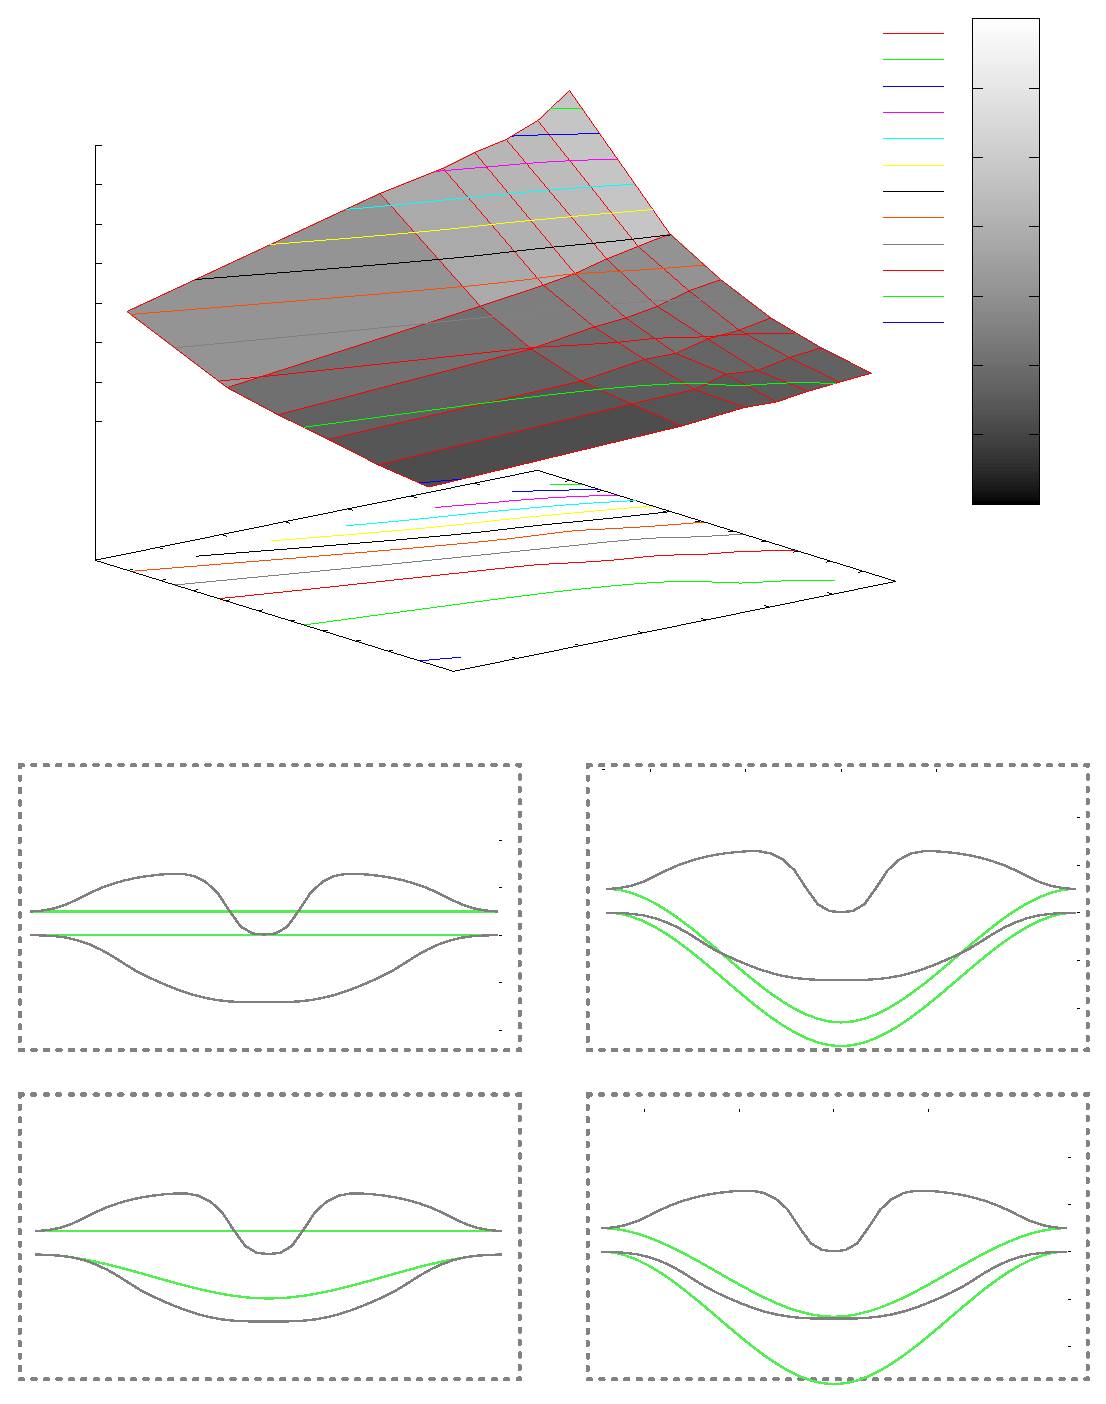
\includegraphics[width=0.9\textwidth]{3dplot_with_sections}
\label{fig:Optimization3dplot}
\end{figure}
%\end{landscape}



%\chapter{Подготовка модели для дальнейших исследований}
%\chapter{Практическая значимость задачи}

В настоящее время всё большее внимание уделяется принципиальной схеме самолета ``летающее крыло''. Данная схема применяется в том числе и для разработки беспилотных летательных аппаратов, предназначенных для разведки. В конструктировании таких самолетов особое внимание уделяется требованиям малозаметности и увеличения аэродинамического качества, и как слествие, возможности барражировать в течение длительного времени. 

Для удовлетворения данным требованиям конструкцию самолета создают максимально ``плоской'' -- так, в подобных конструкциях строительная высота фюзеляжа сравнима с высотой двигателя. Один из способов создания подобной конструкции -- использование изогнутого кессона. (Рис.\ref{fig:OriginalSectionWithEngine}). Примером такого самолета служит концепт американского беспилотного летательного аппарата RQ-180 (Рис.\ref{fig:rq180}). 

\begin{figure}[ht]
\centering
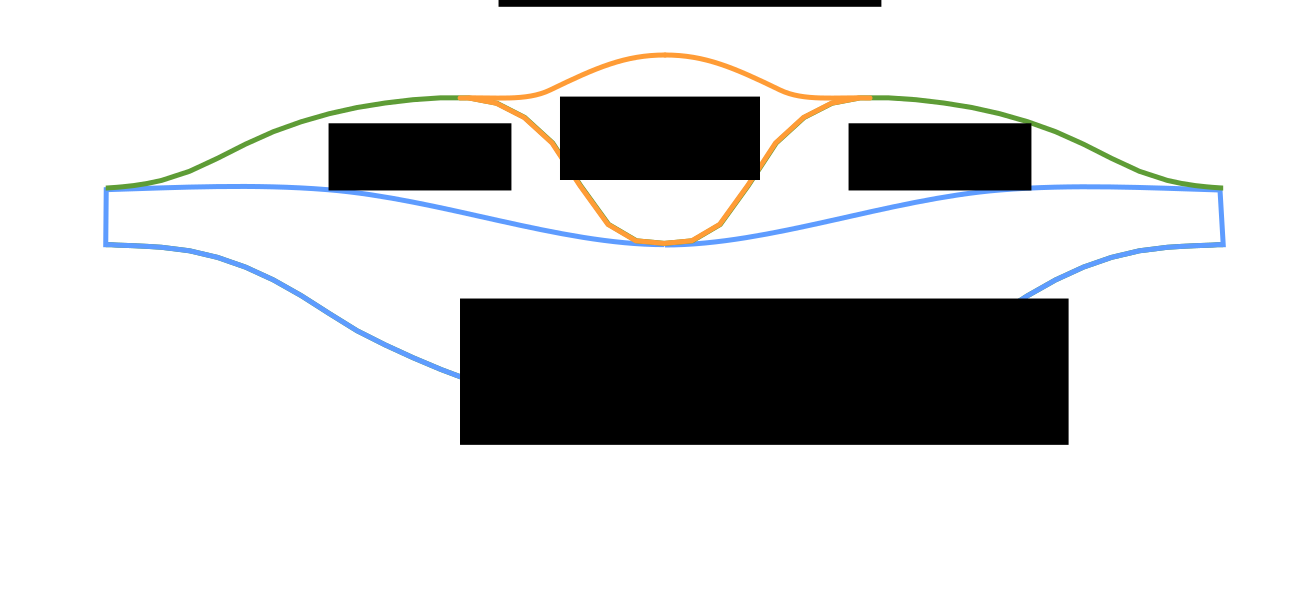
\includegraphics[width=0.7\textwidth]{OriginalSectionWithEngine}
\caption{Вид сечения центроплана в месте стыка передней кромки крыла и фюзеляжа с изображением двигателя}
\label{fig:OriginalSectionWithEngine}
\end{figure}

\begin{figure}[ht]
\centering
\includegraphics[width=0.6\textwidth]{rq180concept}
\caption{Концепт американского БПЛА RQ-180}
\label{fig:rq180}
\end{figure}

Так как вес конструкции является одним из важнейших критериев при выборе конструкции самолета, (что-то дописать), при проектировании самолета необходимо знать, какой вклад в вес конструкции совершает выбор такой формы кессона. С целью получения таких сведений в данной работе проводится анализ влияния различных форм кессона на вес самолета. 

Стоит заметить, что для того, чтобы в полной мере понимать целесообразность выбора той или иной формы центроплана, необходимо проводить комплексный анализ с учетом того, как меняются аэродинамических характеристик самолета при выборе той или иной формы кессона, и выбирать оптимальный вариант, исходя из критериев как прочности, так и аэродинамики. В данной работе проводится анализ лишь с точки зрения прочности конструкции, аэродинамические характеристики и нагрузки приняты постоянными. 

Полученные в работе данные возможно использовать при дальнейшем проектировании самолетов схемы ``летающее крыло''. 
%\chapter{Подготовка к решению задачи}

\section{Программный комплекс ``Conver''}

\subsection{Описание комплекса}
Комплекс представляет собой многоуровневую среду для автоматизированного проектирования и оптимизации ЛА. Комплекс делится на 4 уровня по степени детализации:



\begin{figure}[ht]
\centering
\includegraphics[width=0.6\textwidth]{ConverCircle} 
\caption{Принципиальная схема четырехуровневого проектирования}
\end{figure}



\begin{itemize}
\item Уровень 1: расчёт аэродинамических нагрузок и аэродинамических характеристик; 
\item Уровень 2: расчёт инерционных нагрузок, формирование случаев нагружения, решение задач статической и динамической аэроупругости, анализ веса конструкции планера;
\item Уровень 3: расчёт местной и общей устойчивости, анализ закритического состояния отдельных элементов конструкции, расчёт нелинейного НДС панелей гермокабины, расчет несущей способности элементов конструкции;
\item Уровень 4: расчёт общего НДС конструкции ЛА, определение запасов прочности, определение остаточной прочности, расчет длительной прочности.
\end{itemize}

Основные особенности программного комплекса:

\begin{enumerate}
\item Эффективное проведение параметрических исследований для различных конструкций планера, что позволяет минимизировать временные затраты и снизить трудоёмкость всего процесса;
\item Обеспечение более высокого качественного уровня параметрических исследований на начальной стадии проектирования за счёт автоматизированного создания полноразмерных моделей конструкции ЛА и автоматизации процесса анализа результатов исследований;
\item Оперативная оценка веса конструкций летательных аппаратов с учётом технологических ограничений при автоматическом использовании специализированных баз данных поправочных технологических коэффициентов.
\end{enumerate}


\subsection{Внесенные изменения}

В ходе работы был создан новый интерфейс  для первого уровня комплекса. 

\begin{figure}[h]
\centering
\includegraphics[width=0.8\textwidth]{ConverNewInterfaceOverview}
\caption{Новый интерфейс программного комплекса ``Conver''}
\label{fig:ConverNewInterfaceOverview}
\end{figure}


В новом интерфейсе были реализованы следующие изменения:

\begin{itemize}
	\item Полностью переработана система визуализации
	\begin{itemize}
		\item Добавлены инструменты масштаба и перемещения
		\item Добавлена двусторонняя связь между схемой и областями ввода данных
		\item Добавлена возможность отображения каждого этажа в 		схеме по отдельности
		\item Добавлено отображение ошибок во введенных данных
	\end{itemize}
	\item Переработана система ввода параметров отсеков
	\begin{itemize}
		\item Добавлены визуальные подсказки, предупреждающие ошибки в данных
		\item Добавлена возможность ввода параметров сразу для нескольких отсеков
	\end{itemize}
	\item Добавлена возможность ввода нагрузок непосредственно через задание сил, действующих на отсек
	\item Добавлена возможность просмотра данных, получаемых из других уровней комплекса:
	\begin{itemize}
		\item Оценочный расчет веса конструкции или выбранных отсеков
		\item Расчет объема выбранных отсеков
		\item Просмотр площадей стенок отсеков
	\end{itemize}
\end{itemize}

Рассмотрим, как изменилась работа с типовыми операциями, с которыми приходится сталкиваться пользователю. 


\subsection{Сравнение работы с типовыми операциями в старой и новой версии интерфейса}

\subsubsection{Изменение толщин в отсеке}

Задача: изменить толщину отсека в центроплане. 

\paragraph{Прежний подход:} 

\begin{itemize}
\item Найти номер отсека по схеме (Рис.\ref{fig:ConverListxzOld}) ($\sim1-3~\text{мин.}$)
\item Найти соответствующую ячейку в таблице толщин. ($\sim15~\text{сек.}$)
\item Изменить значение в ячейке. ($\sim5~\text{сек.}$)
\end{itemize}

Итого: $\sim3~\text{мин.}$

\begin{figure}[ht]
\centering
\includegraphics[width=0.8\textwidth]{ConverListxzOld}
\caption{Окно отображения отсеков в предыдущей версии интерфейса}
\label{fig:ConverListxzOld}
\end{figure}

\paragraph{Новый подход:}

\begin{itemize}
\item Кликнуть на нужный отсек на схеме (Рис.\ref($\sim5~\text{сек.}$)
\item Изменить значение в ячейке толщины нужной стенки($\sim5~\text{сек.}$)
\end{itemize}

Итого: $\sim10~\text{сек.}$

\begin{figure}[ht]
\centering
\includegraphics[width=0.8\textwidth]{ConverNewChangingThicks}
\caption{Окно отображения отсеков в новой версии интерфейса}
\label{ConverNewChangingThicks}
\end{figure}

\subsubsection{Нагружение отсека заданной силой}

Задача: по визуальному нахождению стенки нагрузить её заданной силой.

\paragraph{Прежний подход:}

\begin{itemize}
\item Найти по схеме (Рис.\ref{fig:ConverListxzOld}) отсеки, в которых может быть определена нужная стенка ($\sim5~\text{мин.}$)
\item Найти в таблице толщин, какой из выбранных отсеков имеет толщину этой стенки отличную от нуля($\sim3~\text{мин.}$)
\item Из 4 уровня программы найти площадь этой стенки($\sim3~\text{мин.}$)
\item По площади стенки найти давление, которое необходимо на неё приложить($\sim1~\text{мин.}$)
\item В таблице давлений найти нужную ячейку и ввести в неё полученную величину($\sim5~\text{мин.}$)
\end{itemize}

Итого: $\sim17~\text{мин.}$

\paragraph{Новый подход:}

\begin{itemize}
\item Кликнуть на один из отсеков, которому принадлежит эта стенка($\sim10~\text{сек.}$)
\item Если ячейка давления на нужную стенку выделена красным, выбрать другой отсек, в котором эта ячейка не выделена красным, то есть в которой эта стенка имеет ненулевую толщину($\sim1~\text{мин.}$)
\item Нажать кнопку ``Add load''  ($\sim10~\text{сек.}$)
\item В открывшемся окне (Рис.\ref{fig:ConverAddLoad}) ввести величину прикладываемой силы и выбрать стенки отсека, на которые должна быть распределена данная нагрузка. ($\sim30~\text{сек.}$) 
\item Нажать ``Add load'' ($\sim10~\text{сек.}$)

\end{itemize}

Итого: $\sim2~\text{мин.}$

\begin{figure}[ht]
\centering
\includegraphics[width=0.5\textwidth]{ConverNewInterfaceAddLoad}
\caption{Окно добавления нагрузок в новой версии интерфейса}
\label{fig:ConverAddLoad}
\end{figure}
\section{Подбор оптимального размера конечного элемента}

Было построено 7 моделей с различным размером конечного элемента. Путем расчета моделей с заданными нагрузками были определены средние величины напряжений для стенок в наиболее напряженных отсеках (обозначены белым на  Рис.\ref{fig:WingRootPlain})

\begin{figure}[ht]
\centering
\includegraphics[width=0.6\textwidth]{RootOfWingWithSelectedPartsBW}
\caption{Стык правого крыла и фюзеляжа. Схематичное изображение вида сверху}
\label{fig:WingRootPlain}
\end{figure}


\begin{figure}[H]
\centering
\includegraphics[width=0.8\textwidth]{StressToDiscretenessPlot}
\caption{Зависимость средних напряжений в отсеках от величины КЭ}
\label{fig:stressToDiscreteness}
\end{figure}

Была получена зависимость средних напряжений в этих отсеках от размера конечного элемента (Рис.\ref{fig:stressToDiscreteness})

На основании полученных данных была определена оптимальная величина конечного элемента для дальнейшей работы над моделью, равная $0,11\text{м}$. 
%Ниже приведены картины НДС в месте стыка крыла с фюзеляжем при различных размерах конечного элемента. 
%\chapter{Решение задачи}
\section{Создание параметрической модели центроплана}
\label{sec:creationOfModel}

В рамках решения задачи была создана упрощенная параметрическая модель центроплана с двумя варьируемыми  параметрами. В упрощенной модели кессон фюзеляжной части центроплана заменен коробом переменного прямоугольного сечения с поперечными стенками. На короб передаются усилия путем приложения аэродинамических нагрузок на упрощенную модель крыла -- короб постоянного прямоугольного сечения (Рис.\ref{fig:CurvedKessonPatran}). Все панели и стенки считаются алюминиевыми, панели и стенки имеют постоянную толщину по их площади, панели и стенки без вырезов. Носовая и хвостовая части самолёта опущены для простоты расчета.  



\begin{figure}[ht]
\centering
\includegraphics[width=0.9\textwidth]{simplifiedCentroplan}
\caption{Упрощенная модель центроплана с выделением исследуемой части}
\label{fig:CurvedKessonPatran}
\end{figure}

Использование в МКЭ-расчете такой упрощенной модели позволяет значительно ускорить процесс прочностного параметрического анализа при тех же вычислительных мощностях. Так, в упрощенной модели используется $\approx10000$ конечных элементов, в то время как в полной модели самолета используется $\approx270000$ конечных элементов.

Как было сказано выше, рассматриваемая модель имеет два варьируемых параметра: относительная координата нижней точки сечения и строительная высота сечения в плоскости XY в плоскости симметрии самолета. В качестве кривых, описывающих нижнюю и верхнюю поверхность кессона выбраны кубические сплайны, построенные через найденные исходя из выбранных параметров точки. Производные сплайнов в точках стыка фюзеляжа с крылом ($z=2.45\text{м}$) и в плоскости симметрии самолета ($z=0\text{м}$) приняты равными нулю. Пример модельного сечения центроплана в плоскости YZ приведен на Рис.\ref{fig:KessSectionExample}.

\begin{figure}[ht]
\centering
%\def\svgwidth{1\textwidth}
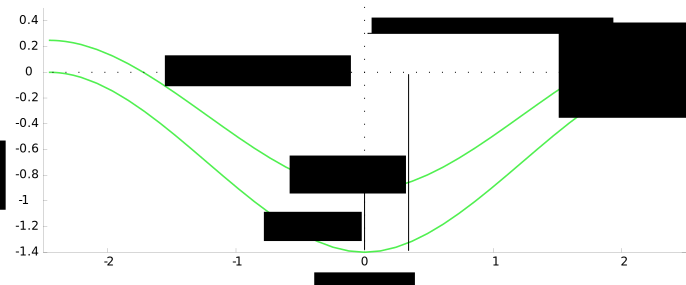
\includegraphics[width=1\textwidth]{KessSectionExample}
%\input{figures/KessSectionExample.pdf_tex}
\caption{Пример модельного поперечного сечения центроплана}
\label{fig:KessSectionExample}
\end{figure}


Выбор такой параметрической модели позволит в дальнейшем (вне рамок данной работы) включить в процесс оптимизации сечения также расчет аэродинамических нагрузок, что позволит полностью автоматизировать процесс оптимизации формы центроплана для центропланов такого типа. 


\section{Оптимизация геометрических параметров сечения центроплана}


\tabulinesep = 1mm
\definecolor{lightgray}{gray}{0.9}
\begin{table}[]
\captionsetup{justification=centering}
\caption{Зависимость площади панелей центроплана и веса кессонаот параметров центроплана}
%\rowcolors{2}{}{lightgray}
\begin{tabu}to \linewidth{|c|*4{X[m c]}|*4{X[m c]}|}
\hline
\multirow{2}{*}[-1.1ex]{N} & \multicolumn{4}{c|}{Площадь панелей} & \multicolumn{4}{c|}{Вес кессона} \\ \cline{2-9}
& Верхние панели & Нижние панели & Боковые стенки & $\Sigma$ & Верхние панели & Нижние панели & Боковые стенки & $\Sigma$ \\
\hline
\taburowcolors {lightgray .. white}
0.000  & 0.249 & 297.182 & 294.551 & 12.561 & 604.294 & 2.730 & 2.730 & 4.000 & 9.520\\ \hline
0.000  & 0.403 & 225.261 & 237.378 & 27.672 & 490.313 & 2.730 & 2.740 & 5.210 & 10.720\\ \hline
0.000  & 0.481 & 190.080 & 222.327 & 49.159 & 461.564 & 2.730 & 2.760 & 5.820 & 11.340\\ \hline
0.000  & 0.558 & 161.544 & 211.467 & 65.963 & 438.972 & 2.730 & 2.760 & 6.450 & 11.950\\ \hline
0.000  & 0.635 & 146.581 & 199.989 & 66.844 & 413.415 & 2.730 & 2.780 & 7.090 & 12.590\\ \hline
0.000  & 0.712 & 134.746 & 191.293 & 70.912 & 396.952 & 2.730 & 2.800 & 7.640 & 13.200\\ \hline
-0.800 & 0.249 & 350.816 & 374.021 & 47.679 & 772.515 & 2.910 & 2.910 & 4.000 & 9.850\\ \hline
-0.800 & 0.403 & 253.752 & 259.311 & 53.180 & 566.245 & 2.910 & 2.850 & 5.210 & 10.990\\ \hline
-0.800 & 0.481 & 213.881 & 226.655 & 57.618 & 498.154 & 2.910 & 2.830 & 5.840 & 11.570\\ \hline
-0.800 & 0.558 & 188.442 & 205.603 & 62.047 & 456.092 & 2.910 & 2.810 & 6.450 & 12.150\\ \hline
-0.800 & 0.635 & 174.466 & 196.192 & 66.506 & 437.164 & 2.910 & 2.780 & 7.090 & 12.770\\ \hline
-0.800 & 0.712 & 154.328 & 195.919 & 70.963 & 421.210 & 2.910 & 2.770 & 7.680 & 13.350\\ \hline
-1.000 & 0.249 & 363.681 & 391.414 & 48.862 & 803.953 & 3.010 & 3.000 & 4.000 & 10.000\\ \hline
-1.000 & 0.403 & 258.118 & 275.555 & 53.209 & 586.883 & 3.010 & 2.930 & 5.230 & 11.160\\ \hline
-1.000 & 0.481 & 225.322 & 238.220 & 57.604 & 521.145 & 3.010 & 2.890 & 5.820 & 11.720\\ \hline
-1.000 & 0.558 & 201.612 & 214.755 & 62.046 & 478.413 & 3.010 & 2.860 & 6.440 & 12.310\\ \hline
-1.000 & 0.635 & 171.877 & 203.370 & 66.418 & 441.665 & 3.010 & 2.840 & 7.050 & 12.900\\ \hline
-1.000 & 0.712 & 163.553 & 201.207 & 70.912 & 435.673 & 3.010 & 2.820 & 7.660 & 13.480\\ \hline
-1.100 & 0.249 & 380.079 & 398.521 & 49.032 & 827.631 & 3.050 & 3.050 & 4.000 & 10.110\\ \hline
-1.100 & 0.403 & 267.143 & 279.590 & 53.134 & 599.866 & 3.050 & 2.980 & 5.210 & 11.240\\ \hline
-1.100 & 0.481 & 231.158 & 238.954 & 57.667 & 527.779 & 3.050 & 2.930 & 5.820 & 11.820\\ \hline
-1.100 & 0.558 & 197.327 & 218.001 & 62.040 & 477.368 & 3.050 & 2.910 & 6.410 & 12.390\\ \hline
-1.100 & 0.635 & 191.553 & 205.935 & 66.481 & 463.971 & 3.050 & 2.870 & 7.070 & 12.980\\ \hline
-1.100 & 0.712 & 158.352 & 203.948 & 70.897 & 433.199 & 3.050 & 2.850 & 7.660 & 13.560\\ \hline
-1.200 & 0.249 & 383.525 & 410.374 & 50.351 & 844.249 & 3.110 & 3.110 & 4.000 & 10.210\\ \hline
-1.200 & 0.403 & 279.228 & 288.331 & 53.186 & 620.745 & 3.110 & 3.030 & 5.210 & 11.350\\ \hline
-1.200 & 0.481 & 233.614 & 249.500 & 57.583 & 540.696 & 3.110 & 2.990 & 5.820 & 11.910\\ \hline
-1.200 & 0.558 & 213.922 & 221.683 & 62.125 & 497.728 & 3.110 & 2.950 & 6.450 & 12.500\\ \hline
-1.200 & 0.635 & 180.457 & 210.067 & 66.523 & 457.046 & 3.110 & 2.920 & 7.070 & 13.070\\ \hline
-1.200 & 0.712 & 167.492 & 205.426 & 71.001 & 443.918 & 3.110 & 2.880 & 7.640 & 13.660\\ \hline
-1.300 & 0.249 & 401.418 & 424.040 & 50.413 & 875.868 & 3.160 & 3.160 & 4.000 & 10.330\\ \hline
-1.300 & 0.403 & 285.115 & 297.451 & 53.649 & 636.214 & 3.160 & 3.070 & 5.230 & 11.470\\ \hline
-1.300 & 0.481 & 251.131 & 255.015 & 57.656 & 563.801 & 3.160 & 3.040 & 5.860 & 12.030\\ \hline
-1.300 & 0.558 & 212.049 & 229.543 & 62.067 & 503.658 & 3.160 & 3.000 & 6.450 & 12.610\\ \hline
-1.300 & 0.635 & 191.030 & 215.968 & 66.550 & 473.548 & 3.160 & 2.970 & 7.070 & 13.170\\ \hline
-1.300 & 0.712 & 170.765 & 209.184 & 70.962 & 450.912 & 3.160 & 2.920 & 7.660 & 13.740\\ \hline
-1.400 & 0.249 & 431.880 & 451.562 & 51.974 & 935.418 & 3.230 & 3.230 & 4.000 & 10.440\\ \hline
-1.400 & 0.403 & 291.199 & 306.178 & 54.263 & 651.640 & 3.230 & 3.130 & 5.210 & 11.560\\ \hline
-1.400 & 0.481 & 253.054 & 265.073 & 57.593 & 575.719 & 3.230 & 3.090 & 5.820 & 12.140\\ \hline
-1.400 & 0.558 & 222.782 & 233.403 & 61.948 & 518.132 & 3.230 & 3.050 & 6.400 & 12.700\\ \hline
-1.400 & 0.635 & 197.192 & 218.301 & 66.423 & 481.917 & 3.230 & 3.020 & 7.030 & 13.270\\ \hline
-1.400 & 0.712 & 175.591 & 210.828 & 70.877 & 457.295 & 3.230 & 2.970 & 7.660 & 13.840\\ \hline

\end{tabu}

\end{table}



%\input{sections/validationOfPants}
%\chapter{Валидация решения}


В ходе работы была проведена валидация полученного решения. Валидация проводилась путем сравнения результатов расчета модельной задачи и расчета самолета в целом. 

\begin{table}[ht]
\caption{Сравнение результатов расчета модельной задачи и самолета в целом}
\label{tab:ComparingResults}
\begin{tabu}to \linewidth{|X[m c]|X[m c]|X[m c]|}
\hline
& Результат из расчета модельной задачи & Результат из расчета самолета в целом\\ \hline
Вес обшивки кессона[кг] & 180 & 47 \\ \hline


\end{tabu}
\end{table}


%\chapter{Все разделы}
%\section{Расчет параметрической модели}

Для проведения расчета были выбраны 42 пары значений параметров. Для каждой пары была проведена оптимизация толщин панелей кессона с целью удовлетворения требованиям прочности конструкции, а именно: среднее напряжение в каждой панели не должно превышать значения допускаемого напряжения, принятого равным $35\text{кг}/\text{мм}^2$. Оптимизация проводилась путем вычисления запаса прочности для каждой пластины с последующим делением толщины панели на полученное значение (так называемый алгоритм $\sigma/\sigma$). Итоговые результаты вычислений приведены в таблицах \ref{tab:KessOptimBigTable}, \ref{tab:KessOptimBigTableNormed} и на Рис.\ref{fig:Optimization3dplot} (серым цветом на изображениях сечений показано оригинальное сечение кессона, зеленым - сечение в параметрической модели)  

\tabulinesep = 1mm
\definecolor{lightgray}{gray}{0.9}
\begin{table}[H]
\captionsetup{justification=centering}
\caption{Зависимость площади панелей центроплана и веса кессона от параметров центроплана}
%\rowcolors{2}{}{lightgray}
\begin{tabu}to \linewidth{|c|*4{X[m c]|}*4{X[m c]|}}
\hline
\multirow{2}{*}[-1.1ex]{N} & \multicolumn{4}{c|}{Вес кессона~[кг]} & \multicolumn{4}{c|}{Площадь панелей центроплана~[$\text{м}^2$]} \\ \cline{2-9}
& Верхние панели & Нижние панели & Боковые стенки & $\Sigma$ & Верхние панели & Нижние панели & Боковые стенки & $\Sigma$ \\
\hline
\taburowcolors {lightgray .. white}
0.000  & 0.249 & 297.182 & 294.551 & 12.561 & 604.294 & 2.730 & 2.730 & 4.000 & 9.520\\ \hline
0.000  & 0.403 & 225.261 & 237.378 & 27.672 & 490.313 & 2.730 & 2.740 & 5.210 & 10.720\\ \hline
0.000  & 0.481 & 190.080 & 222.327 & 49.159 & 461.564 & 2.730 & 2.760 & 5.820 & 11.340\\ \hline
0.000  & 0.558 & 161.544 & 211.467 & 65.963 & 438.972 & 2.730 & 2.760 & 6.450 & 11.950\\ \hline
0.000  & 0.635 & 146.581 & 199.989 & 66.844 & 413.415 & 2.730 & 2.780 & 7.090 & 12.590\\ \hline
0.000  & 0.712 & 134.746 & 191.293 & 70.912 & 396.952 & 2.730 & 2.800 & 7.640 & 13.200\\ \hline
-0.800 & 0.249 & 350.816 & 374.021 & 47.679 & 772.515 & 2.910 & 2.910 & 4.000 & 9.850\\ \hline
-0.800 & 0.403 & 253.752 & 259.311 & 53.180 & 566.245 & 2.910 & 2.850 & 5.210 & 10.990\\ \hline
-0.800 & 0.481 & 213.881 & 226.655 & 57.618 & 498.154 & 2.910 & 2.830 & 5.840 & 11.570\\ \hline
-0.800 & 0.558 & 188.442 & 205.603 & 62.047 & 456.092 & 2.910 & 2.810 & 6.450 & 12.150\\ \hline
-0.800 & 0.635 & 174.466 & 196.192 & 66.506 & 437.164 & 2.910 & 2.780 & 7.090 & 12.770\\ \hline
-0.800 & 0.712 & 154.328 & 195.919 & 70.963 & 421.210 & 2.910 & 2.770 & 7.680 & 13.350\\ \hline
-1.000 & 0.249 & 363.681 & 391.414 & 48.862 & 803.953 & 3.010 & 3.000 & 4.000 & 10.000\\ \hline
-1.000 & 0.403 & 258.118 & 275.555 & 53.209 & 586.883 & 3.010 & 2.930 & 5.230 & 11.160\\ \hline
-1.000 & 0.481 & 225.322 & 238.220 & 57.604 & 521.145 & 3.010 & 2.890 & 5.820 & 11.720\\ \hline
-1.000 & 0.558 & 201.612 & 214.755 & 62.046 & 478.413 & 3.010 & 2.860 & 6.440 & 12.310\\ \hline
-1.000 & 0.635 & 171.877 & 203.370 & 66.418 & 441.665 & 3.010 & 2.840 & 7.050 & 12.900\\ \hline
-1.000 & 0.712 & 163.553 & 201.207 & 70.912 & 435.673 & 3.010 & 2.820 & 7.660 & 13.480\\ \hline
-1.100 & 0.249 & 380.079 & 398.521 & 49.032 & 827.631 & 3.050 & 3.050 & 4.000 & 10.110\\ \hline
-1.100 & 0.403 & 267.143 & 279.590 & 53.134 & 599.866 & 3.050 & 2.980 & 5.210 & 11.240\\ \hline
-1.100 & 0.481 & 231.158 & 238.954 & 57.667 & 527.779 & 3.050 & 2.930 & 5.820 & 11.820\\ \hline
-1.100 & 0.558 & 197.327 & 218.001 & 62.040 & 477.368 & 3.050 & 2.910 & 6.410 & 12.390\\ \hline
-1.100 & 0.635 & 191.553 & 205.935 & 66.481 & 463.971 & 3.050 & 2.870 & 7.070 & 12.980\\ \hline
-1.100 & 0.712 & 158.352 & 203.948 & 70.897 & 433.199 & 3.050 & 2.850 & 7.660 & 13.560\\ \hline
-1.200 & 0.249 & 383.525 & 410.374 & 50.351 & 844.249 & 3.110 & 3.110 & 4.000 & 10.210\\ \hline
-1.200 & 0.403 & 279.228 & 288.331 & 53.186 & 620.745 & 3.110 & 3.030 & 5.210 & 11.350\\ \hline
-1.200 & 0.481 & 233.614 & 249.500 & 57.583 & 540.696 & 3.110 & 2.990 & 5.820 & 11.910\\ \hline
-1.200 & 0.558 & 213.922 & 221.683 & 62.125 & 497.728 & 3.110 & 2.950 & 6.450 & 12.500\\ \hline
-1.200 & 0.635 & 180.457 & 210.067 & 66.523 & 457.046 & 3.110 & 2.920 & 7.070 & 13.070\\ \hline
-1.200 & 0.712 & 167.492 & 205.426 & 71.001 & 443.918 & 3.110 & 2.880 & 7.640 & 13.660\\ \hline
-1.300 & 0.249 & 401.418 & 424.040 & 50.413 & 875.868 & 3.160 & 3.160 & 4.000 & 10.330\\ \hline
-1.300 & 0.403 & 285.115 & 297.451 & 53.649 & 636.214 & 3.160 & 3.070 & 5.230 & 11.470\\ \hline
-1.300 & 0.481 & 251.131 & 255.015 & 57.656 & 563.801 & 3.160 & 3.040 & 5.860 & 12.030\\ \hline
-1.300 & 0.558 & 212.049 & 229.543 & 62.067 & 503.658 & 3.160 & 3.000 & 6.450 & 12.610\\ \hline
-1.300 & 0.635 & 191.030 & 215.968 & 66.550 & 473.548 & 3.160 & 2.970 & 7.070 & 13.170\\ \hline
-1.300 & 0.712 & 170.765 & 209.184 & 70.962 & 450.912 & 3.160 & 2.920 & 7.660 & 13.740\\ \hline
-1.400 & 0.249 & 431.880 & 451.562 & 51.974 & 935.418 & 3.230 & 3.230 & 4.000 & 10.440\\ \hline
-1.400 & 0.403 & 291.199 & 306.178 & 54.263 & 651.640 & 3.230 & 3.130 & 5.210 & 11.560\\ \hline
-1.400 & 0.481 & 253.054 & 265.073 & 57.593 & 575.719 & 3.230 & 3.090 & 5.820 & 12.140\\ \hline
-1.400 & 0.558 & 222.782 & 233.403 & 61.948 & 518.132 & 3.230 & 3.050 & 6.400 & 12.700\\ \hline
-1.400 & 0.635 & 197.192 & 218.301 & 66.423 & 481.917 & 3.230 & 3.020 & 7.030 & 13.270\\ \hline
-1.400 & 0.712 & 175.591 & 210.828 & 70.877 & 457.295 & 3.230 & 2.970 & 7.660 & 13.840\\ \hline

\end{tabu}

\label{tab:KessOptimBigTable}
\end{table}


\tabulinesep = 1mm
\definecolor{lightgray}{gray}{0.9}
\begin{table}[H]
\captionsetup{justification=centering}
\caption{Зависимость площади панелей центроплана и веса кессона от параметров центроплана относительно варианта с прямым кессоном}
%\rowcolors{2}{}{lightgray}
\begin{tabu}to \linewidth{|c|*4{X[m c]|}*4{X[m c]|}}
\hline
\multirow{2}{*}[-1.1ex]{N} & \multicolumn{4}{c|}{Вес кессона} & \multicolumn{4}{c|}{Площадь панелей центроплана} \\ \cline{2-9}
& Верхние панели & Нижние панели & Боковые стенки & $\Sigma$ & Верхние панели & Нижние панели & Боковые стенки & $\Sigma$ \\
\hline
\taburowcolors {lightgray .. white}
0.000  & 0.249 & 0.492 & 0.487 & 0.021 & 1.000 & 0.287 & 0.287 & 0.420 & 1.000\\ \hline
0.000  & 0.403 & 0.373 & 0.393 & 0.046 & 0.811 & 0.287 & 0.288 & 0.547 & 1.126\\ \hline
0.000  & 0.481 & 0.315 & 0.368 & 0.081 & 0.764 & 0.287 & 0.290 & 0.611 & 1.191\\ \hline
0.000  & 0.558 & 0.267 & 0.350 & 0.109 & 0.726 & 0.287 & 0.290 & 0.678 & 1.255\\ \hline
0.000  & 0.635 & 0.243 & 0.331 & 0.111 & 0.684 & 0.287 & 0.292 & 0.745 & 1.322\\ \hline
0.000  & 0.712 & 0.223 & 0.317 & 0.117 & 0.657 & 0.287 & 0.294 & 0.803 & 1.387\\ \hline \hline
-0.800 & 0.249 & 0.581 & 0.619 & 0.079 & 1.278 & 0.306 & 0.306 & 0.420 & 1.035\\ \hline
-0.800 & 0.403 & 0.420 & 0.429 & 0.088 & 0.937 & 0.306 & 0.299 & 0.547 & 1.154\\ \hline
-0.800 & 0.481 & 0.354 & 0.375 & 0.095 & 0.824 & 0.306 & 0.297 & 0.613 & 1.215\\ \hline
-0.800 & 0.558 & 0.312 & 0.340 & 0.103 & 0.755 & 0.306 & 0.295 & 0.678 & 1.276\\ \hline
-0.800 & 0.635 & 0.289 & 0.325 & 0.110 & 0.723 & 0.306 & 0.292 & 0.745 & 1.341\\ \hline
-0.800 & 0.712 & 0.255 & 0.324 & 0.117 & 0.697 & 0.306 & 0.291 & 0.807 & 1.402\\ \hline \hline
-1.000 & 0.249 & 0.602 & 0.648 & 0.081 & 1.330 & 0.316 & 0.315 & 0.420 & 1.050\\ \hline
-1.000 & 0.403 & 0.427 & 0.456 & 0.088 & 0.971 & 0.316 & 0.308 & 0.549 & 1.172\\ \hline
-1.000 & 0.481 & 0.373 & 0.394 & 0.095 & 0.862 & 0.316 & 0.304 & 0.611 & 1.231\\ \hline
-1.000 & 0.558 & 0.334 & 0.355 & 0.103 & 0.792 & 0.316 & 0.300 & 0.676 & 1.293\\ \hline
-1.000 & 0.635 & 0.284 & 0.337 & 0.110 & 0.731 & 0.316 & 0.298 & 0.741 & 1.355\\ \hline
-1.000 & 0.712 & 0.271 & 0.333 & 0.117 & 0.721 & 0.316 & 0.296 & 0.805 & 1.416\\ \hline \hline
-1.100 & 0.249 & 0.629 & 0.659 & 0.081 & 1.370 & 0.320 & 0.320 & 0.420 & 1.062\\ \hline
-1.100 & 0.403 & 0.442 & 0.463 & 0.088 & 0.993 & 0.320 & 0.313 & 0.547 & 1.181\\ \hline
-1.100 & 0.481 & 0.383 & 0.395 & 0.095 & 0.873 & 0.320 & 0.308 & 0.611 & 1.242\\ \hline
-1.100 & 0.558 & 0.327 & 0.361 & 0.103 & 0.790 & 0.320 & 0.306 & 0.673 & 1.301\\ \hline
-1.100 & 0.635 & 0.317 & 0.341 & 0.110 & 0.768 & 0.320 & 0.301 & 0.743 & 1.363\\ \hline
-1.100 & 0.712 & 0.262 & 0.337 & 0.117 & 0.717 & 0.320 & 0.299 & 0.805 & 1.424\\ \hline \hline 
-1.200 & 0.249 & 0.635 & 0.679 & 0.083 & 1.397 & 0.327 & 0.327 & 0.420 & 1.072\\ \hline
-1.200 & 0.403 & 0.462 & 0.477 & 0.088 & 1.027 & 0.327 & 0.318 & 0.547 & 1.192\\ \hline
-1.200 & 0.481 & 0.387 & 0.413 & 0.095 & 0.895 & 0.327 & 0.314 & 0.611 & 1.251\\ \hline
-1.200 & 0.558 & 0.354 & 0.367 & 0.103 & 0.824 & 0.327 & 0.310 & 0.678 & 1.313\\ \hline
-1.200 & 0.635 & 0.299 & 0.348 & 0.110 & 0.756 & 0.327 & 0.307 & 0.743 & 1.373\\ \hline
-1.200 & 0.712 & 0.277 & 0.340 & 0.117 & 0.735 & 0.327 & 0.303 & 0.803 & 1.435\\ \hline \hline
-1.300 & 0.249 & 0.664 & 0.702 & 0.083 & 1.449 & 0.332 & 0.332 & 0.420 & 1.085\\ \hline
-1.300 & 0.403 & 0.472 & 0.492 & 0.089 & 1.053 & 0.332 & 0.322 & 0.549 & 1.205\\ \hline
-1.300 & 0.481 & 0.416 & 0.422 & 0.095 & 0.933 & 0.332 & 0.319 & 0.616 & 1.264\\ \hline
-1.300 & 0.558 & 0.351 & 0.380 & 0.103 & 0.833 & 0.332 & 0.315 & 0.678 & 1.325\\ \hline
-1.300 & 0.635 & 0.316 & 0.357 & 0.110 & 0.784 & 0.332 & 0.312 & 0.743 & 1.383\\ \hline
-1.300 & 0.712 & 0.283 & 0.346 & 0.117 & 0.746 & 0.332 & 0.307 & 0.805 & 1.443\\ \hline \hline
-1.400 & 0.249 & 0.715 & 0.747 & 0.086 & 1.548 & 0.339 & 0.339 & 0.420 & 1.097\\ \hline
-1.400 & 0.403 & 0.482 & 0.507 & 0.090 & 1.078 & 0.339 & 0.329 & 0.547 & 1.214\\ \hline
-1.400 & 0.481 & 0.419 & 0.439 & 0.095 & 0.953 & 0.339 & 0.325 & 0.611 & 1.275\\ \hline
-1.400 & 0.558 & 0.369 & 0.386 & 0.103 & 0.857 & 0.339 & 0.320 & 0.672 & 1.334\\ \hline
-1.400 & 0.635 & 0.326 & 0.361 & 0.110 & 0.797 & 0.339 & 0.317 & 0.738 & 1.394\\ \hline
-1.400 & 0.712 & 0.291 & 0.349 & 0.117 & 0.757 & 0.339 & 0.312 & 0.805 & 1.454\\ \hline

\end{tabu}

\label{tab:KessOptimBigTableNormed}
\end{table}

%\begin{landscape}
\begin{figure}[ht]
\captionsetup{justification=centering}
\caption{Зависимость веса кессона от параметров центроплана}
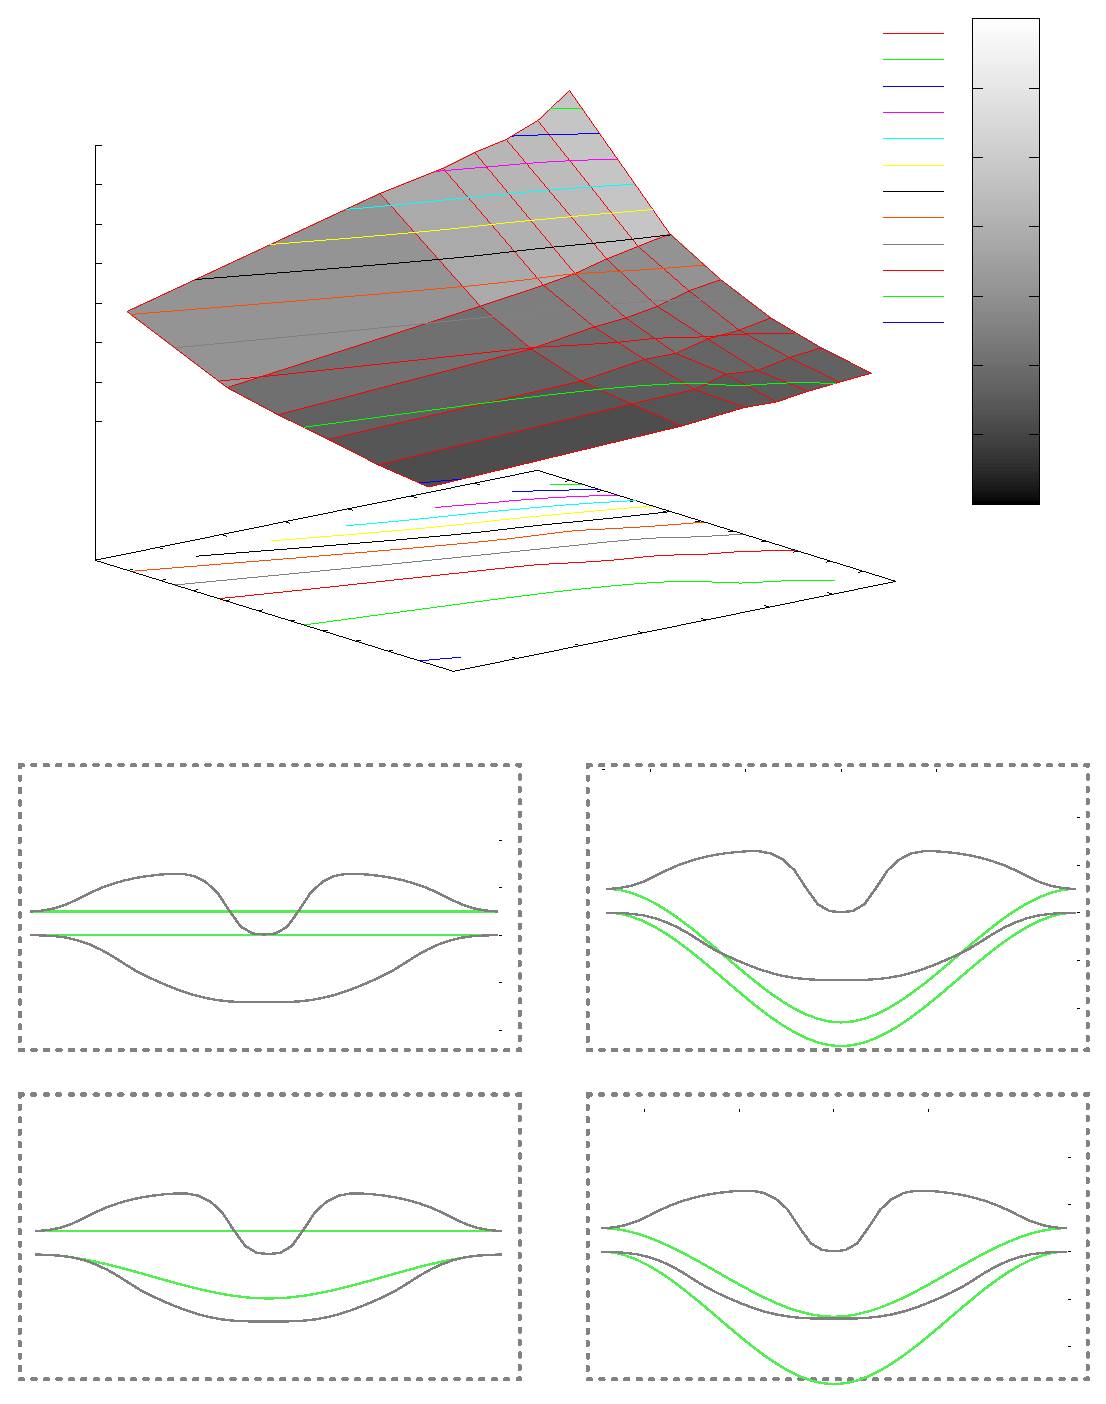
\includegraphics[width=0.9\textwidth]{3dplot_with_sections}
\label{fig:Optimization3dplot}
\end{figure}
%\end{landscape}



%%\section{Создание конечно-элементной модели проектируемого самолета}

В ходе работы были исследованы вопросы построения проектировочной модели БПЛА с крылом большого удлинения и несущим фюзеляжем. При помощи программного комплекса ``Conver'' (см. раздел \ref{sec:Conver}), исходя из взятой за основу концептуальной модели, была создана МКЭ-модель проектируемого БПЛА с исключенной верхней частью воздухозаборника, не несущей в себе силовых элементов. 

%\begin{figure}[ht]
%\centering
%\includegraphics[width=0.8\textwidth]{BPLAfullModel}
%\caption{МКЭ-модель проектируемого БПЛА без верхней части}
%\label{fig:BPLAfullModel}
%\end{figure}

\subsection{Требования к прочностной модели}

К прочностной модели предъявляются следующие требования:

\begin{enumerate}
\item оперативность построения модели
\item подробность модели
\item надежность анализа
\item возможность модификации 
\item рациональный выбор конечно-элементной сетки
\end{enumerate}

%Выбор базового комплекса
\subsection{Выбор базового комплекса}
Учитывая представленные выше требования к модели, для построения моделей в работе был использован программный комплекс ``Conver'', разработанный в НИО-3 ЦАГИ. 
% в описании конвера расписывать, чем он нам подходит
%\subsection{Программный комплекс ``Conver''}
\label{sec:Conver}

Для построения описанных выше моделей использовался разработанный в ЦАГИ программный комплекс ``Conver''. Его использование позволило многократно сократить время построения каждой модели. 

%\subsection{Описание комплекса}
Комплекс представляет собой многоуровневую среду для автоматизированного проектирования и оптимизации ЛА. Комплекс делится на 4 уровня по степени детализации:



\begin{figure}[ht]
\centering
\includegraphics[width=0.6\textwidth]{ConverCircle} 
\caption{Принципиальная схема четырехуровневого проектирования}
\end{figure}



\begin{itemize}
\item Уровень 1: расчёт аэродинамических нагрузок и аэродинамических характеристик; 
\item Уровень 2: расчёт инерционных нагрузок, формирование случаев нагружения, решение задач статической и динамической аэроупругости, анализ веса конструкции планера;
\item Уровень 3: расчёт местной и общей устойчивости, анализ закритического состояния отдельных элементов конструкции, расчёт нелинейного НДС панелей гермокабины, расчет несущей способности элементов конструкции;
\item Уровень 4: расчёт общего НДС конструкции ЛА, определение запасов прочности, определение остаточной прочности, расчет длительной прочности.
\end{itemize}

Основные особенности программного комплекса:

\begin{enumerate}
\item Эффективное проведение параметрических исследований для различных конструкций планера, что позволяет минимизировать временные затраты и снизить трудоёмкость всего процесса;
\item Обеспечение более высокого качественного уровня параметрических исследований на начальной стадии проектирования за счёт автоматизированного создания полноразмерных моделей конструкции ЛА и автоматизации процесса анализа результатов исследований;
\item Оперативная оценка веса конструкций летательных аппаратов с учётом технологических ограничений при автоматическом использовании специализированных баз данных поправочных технологических коэффициентов.
\end{enumerate}

%Нарисовать блок-схему взаимодействия nastran patran conver расчетная модель автокад аэродинамика


%\section{Программный комплекс ``Conver''}

\subsection{Описание комплекса}
Комплекс представляет собой многоуровневую среду для автоматизированного проектирования и оптимизации ЛА. Комплекс делится на 4 уровня по степени детализации:



\begin{figure}[ht]
\centering
\includegraphics[width=0.6\textwidth]{ConverCircle} 
\caption{Принципиальная схема четырехуровневого проектирования}
\end{figure}



\begin{itemize}
\item Уровень 1: расчёт аэродинамических нагрузок и аэродинамических характеристик; 
\item Уровень 2: расчёт инерционных нагрузок, формирование случаев нагружения, решение задач статической и динамической аэроупругости, анализ веса конструкции планера;
\item Уровень 3: расчёт местной и общей устойчивости, анализ закритического состояния отдельных элементов конструкции, расчёт нелинейного НДС панелей гермокабины, расчет несущей способности элементов конструкции;
\item Уровень 4: расчёт общего НДС конструкции ЛА, определение запасов прочности, определение остаточной прочности, расчет длительной прочности.
\end{itemize}

Основные особенности программного комплекса:

\begin{enumerate}
\item Эффективное проведение параметрических исследований для различных конструкций планера, что позволяет минимизировать временные затраты и снизить трудоёмкость всего процесса;
\item Обеспечение более высокого качественного уровня параметрических исследований на начальной стадии проектирования за счёт автоматизированного создания полноразмерных моделей конструкции ЛА и автоматизации процесса анализа результатов исследований;
\item Оперативная оценка веса конструкций летательных аппаратов с учётом технологических ограничений при автоматическом использовании специализированных баз данных поправочных технологических коэффициентов.
\end{enumerate}


\subsection{Внесенные изменения}

В ходе работы был создан новый интерфейс  для первого уровня комплекса. 

\begin{figure}[h]
\centering
\includegraphics[width=0.8\textwidth]{ConverNewInterfaceOverview}
\caption{Новый интерфейс программного комплекса ``Conver''}
\label{fig:ConverNewInterfaceOverview}
\end{figure}


В новом интерфейсе были реализованы следующие изменения:

\begin{itemize}
	\item Полностью переработана система визуализации
	\begin{itemize}
		\item Добавлены инструменты масштаба и перемещения
		\item Добавлена двусторонняя связь между схемой и областями ввода данных
		\item Добавлена возможность отображения каждого этажа в 		схеме по отдельности
		\item Добавлено отображение ошибок во введенных данных
	\end{itemize}
	\item Переработана система ввода параметров отсеков
	\begin{itemize}
		\item Добавлены визуальные подсказки, предупреждающие ошибки в данных
		\item Добавлена возможность ввода параметров сразу для нескольких отсеков
	\end{itemize}
	\item Добавлена возможность ввода нагрузок непосредственно через задание сил, действующих на отсек
	\item Добавлена возможность просмотра данных, получаемых из других уровней комплекса:
	\begin{itemize}
		\item Оценочный расчет веса конструкции или выбранных отсеков
		\item Расчет объема выбранных отсеков
		\item Просмотр площадей стенок отсеков
	\end{itemize}
\end{itemize}

Рассмотрим, как изменилась работа с типовыми операциями, с которыми приходится сталкиваться пользователю. 


\subsection{Сравнение работы с типовыми операциями в старой и новой версии интерфейса}

\subsubsection{Изменение толщин в отсеке}

Задача: изменить толщину отсека в центроплане. 

\paragraph{Прежний подход:} 

\begin{itemize}
\item Найти номер отсека по схеме (Рис.\ref{fig:ConverListxzOld}) ($\sim1-3~\text{мин.}$)
\item Найти соответствующую ячейку в таблице толщин. ($\sim15~\text{сек.}$)
\item Изменить значение в ячейке. ($\sim5~\text{сек.}$)
\end{itemize}

Итого: $\sim3~\text{мин.}$

\begin{figure}[ht]
\centering
\includegraphics[width=0.8\textwidth]{ConverListxzOld}
\caption{Окно отображения отсеков в предыдущей версии интерфейса}
\label{fig:ConverListxzOld}
\end{figure}

\paragraph{Новый подход:}

\begin{itemize}
\item Кликнуть на нужный отсек на схеме (Рис.\ref($\sim5~\text{сек.}$)
\item Изменить значение в ячейке толщины нужной стенки($\sim5~\text{сек.}$)
\end{itemize}

Итого: $\sim10~\text{сек.}$

\begin{figure}[ht]
\centering
\includegraphics[width=0.8\textwidth]{ConverNewChangingThicks}
\caption{Окно отображения отсеков в новой версии интерфейса}
\label{ConverNewChangingThicks}
\end{figure}

\subsubsection{Нагружение отсека заданной силой}

Задача: по визуальному нахождению стенки нагрузить её заданной силой.

\paragraph{Прежний подход:}

\begin{itemize}
\item Найти по схеме (Рис.\ref{fig:ConverListxzOld}) отсеки, в которых может быть определена нужная стенка ($\sim5~\text{мин.}$)
\item Найти в таблице толщин, какой из выбранных отсеков имеет толщину этой стенки отличную от нуля($\sim3~\text{мин.}$)
\item Из 4 уровня программы найти площадь этой стенки($\sim3~\text{мин.}$)
\item По площади стенки найти давление, которое необходимо на неё приложить($\sim1~\text{мин.}$)
\item В таблице давлений найти нужную ячейку и ввести в неё полученную величину($\sim5~\text{мин.}$)
\end{itemize}

Итого: $\sim17~\text{мин.}$

\paragraph{Новый подход:}

\begin{itemize}
\item Кликнуть на один из отсеков, которому принадлежит эта стенка($\sim10~\text{сек.}$)
\item Если ячейка давления на нужную стенку выделена красным, выбрать другой отсек, в котором эта ячейка не выделена красным, то есть в которой эта стенка имеет ненулевую толщину($\sim1~\text{мин.}$)
\item Нажать кнопку ``Add load''  ($\sim10~\text{сек.}$)
\item В открывшемся окне (Рис.\ref{fig:ConverAddLoad}) ввести величину прикладываемой силы и выбрать стенки отсека, на которые должна быть распределена данная нагрузка. ($\sim30~\text{сек.}$) 
\item Нажать ``Add load'' ($\sim10~\text{сек.}$)

\end{itemize}

Итого: $\sim2~\text{мин.}$

\begin{figure}[ht]
\centering
\includegraphics[width=0.5\textwidth]{ConverNewInterfaceAddLoad}
\caption{Окно добавления нагрузок в новой версии интерфейса}
\label{fig:ConverAddLoad}
\end{figure}

\subsection{Создание модели}
\label{sec:creationOfOneModel}
\subsubsection{Создание геометрии}
Показать скриншоты из List1,2,4,
\subsubsection{Задание нагрузок и свойств отсеков}
Показать скриншот из ListAdd
\subsubsection{Построение МКЭ-модели}
Показать скриншот из ListA, скрин из патрана. 


%\section{Создание параметрической модели центроплана}
\label{sec:creationOfModel}

В рамках решения задачи была создана упрощенная параметрическая модель центроплана с двумя варьируемыми  параметрами. В упрощенной модели кессон фюзеляжной части центроплана заменен коробом переменного прямоугольного сечения с поперечными стенками. На короб передаются усилия путем приложения аэродинамических нагрузок на упрощенную модель крыла -- короб постоянного прямоугольного сечения (Рис.\ref{fig:CurvedKessonPatran}). Все панели и стенки считаются алюминиевыми, панели и стенки имеют постоянную толщину по их площади, панели и стенки без вырезов. Носовая и хвостовая части самолёта опущены для простоты расчета.  



\begin{figure}[ht]
\centering
\includegraphics[width=0.9\textwidth]{simplifiedCentroplan}
\caption{Упрощенная модель центроплана с выделением исследуемой части}
\label{fig:CurvedKessonPatran}
\end{figure}

Использование в МКЭ-расчете такой упрощенной модели позволяет значительно ускорить процесс прочностного параметрического анализа при тех же вычислительных мощностях. Так, в упрощенной модели используется $\approx10000$ конечных элементов, в то время как в полной модели самолета используется $\approx270000$ конечных элементов.

Как было сказано выше, рассматриваемая модель имеет два варьируемых параметра: относительная координата нижней точки сечения и строительная высота сечения в плоскости XY в плоскости симметрии самолета. В качестве кривых, описывающих нижнюю и верхнюю поверхность кессона выбраны кубические сплайны, построенные через найденные исходя из выбранных параметров точки. Производные сплайнов в точках стыка фюзеляжа с крылом ($z=2.45\text{м}$) и в плоскости симметрии самолета ($z=0\text{м}$) приняты равными нулю. Пример модельного сечения центроплана в плоскости YZ приведен на Рис.\ref{fig:KessSectionExample}.

\begin{figure}[ht]
\centering
%\def\svgwidth{1\textwidth}
\includegraphics[width=1\textwidth]{KessSectionExample}
%\input{figures/KessSectionExample.pdf_tex}
\caption{Пример модельного поперечного сечения центроплана}
\label{fig:KessSectionExample}
\end{figure}


Выбор такой параметрической модели позволит в дальнейшем (вне рамок данной работы) включить в процесс оптимизации сечения также расчет аэродинамических нагрузок, что позволит полностью автоматизировать процесс оптимизации формы центроплана для центропланов такого типа. 


%\section{Подбор оптимального размера конечного элемента}

Было построено 7 моделей с различным размером конечного элемента. Путем расчета моделей с заданными нагрузками были определены средние величины напряжений для стенок в наиболее напряженных отсеках (обозначены белым на  Рис.\ref{fig:WingRootPlain})

\begin{figure}[ht]
\centering
\includegraphics[width=0.6\textwidth]{RootOfWingWithSelectedPartsBW}
\caption{Стык правого крыла и фюзеляжа. Схематичное изображение вида сверху}
\label{fig:WingRootPlain}
\end{figure}


\begin{figure}[H]
\centering
\includegraphics[width=0.8\textwidth]{StressToDiscretenessPlot}
\caption{Зависимость средних напряжений в отсеках от величины КЭ}
\label{fig:stressToDiscreteness}
\end{figure}

Была получена зависимость средних напряжений в этих отсеках от размера конечного элемента (Рис.\ref{fig:stressToDiscreteness})

На основании полученных данных была определена оптимальная величина конечного элемента для дальнейшей работы над моделью, равная $0,11\text{м}$. 
%Ниже приведены картины НДС в месте стыка крыла с фюзеляжем при различных размерах конечного элемента. 
%\section{Оптимизация геометрических параметров сечения центроплана}


\tabulinesep = 1mm
\definecolor{lightgray}{gray}{0.9}
\begin{table}[]
\captionsetup{justification=centering}
\caption{Зависимость площади панелей центроплана и веса кессонаот параметров центроплана}
%\rowcolors{2}{}{lightgray}
\begin{tabu}to \linewidth{|c|*4{X[m c]}|*4{X[m c]}|}
\hline
\multirow{2}{*}[-1.1ex]{N} & \multicolumn{4}{c|}{Площадь панелей} & \multicolumn{4}{c|}{Вес кессона} \\ \cline{2-9}
& Верхние панели & Нижние панели & Боковые стенки & $\Sigma$ & Верхние панели & Нижние панели & Боковые стенки & $\Sigma$ \\
\hline
\taburowcolors {lightgray .. white}
0.000  & 0.249 & 297.182 & 294.551 & 12.561 & 604.294 & 2.730 & 2.730 & 4.000 & 9.520\\ \hline
0.000  & 0.403 & 225.261 & 237.378 & 27.672 & 490.313 & 2.730 & 2.740 & 5.210 & 10.720\\ \hline
0.000  & 0.481 & 190.080 & 222.327 & 49.159 & 461.564 & 2.730 & 2.760 & 5.820 & 11.340\\ \hline
0.000  & 0.558 & 161.544 & 211.467 & 65.963 & 438.972 & 2.730 & 2.760 & 6.450 & 11.950\\ \hline
0.000  & 0.635 & 146.581 & 199.989 & 66.844 & 413.415 & 2.730 & 2.780 & 7.090 & 12.590\\ \hline
0.000  & 0.712 & 134.746 & 191.293 & 70.912 & 396.952 & 2.730 & 2.800 & 7.640 & 13.200\\ \hline
-0.800 & 0.249 & 350.816 & 374.021 & 47.679 & 772.515 & 2.910 & 2.910 & 4.000 & 9.850\\ \hline
-0.800 & 0.403 & 253.752 & 259.311 & 53.180 & 566.245 & 2.910 & 2.850 & 5.210 & 10.990\\ \hline
-0.800 & 0.481 & 213.881 & 226.655 & 57.618 & 498.154 & 2.910 & 2.830 & 5.840 & 11.570\\ \hline
-0.800 & 0.558 & 188.442 & 205.603 & 62.047 & 456.092 & 2.910 & 2.810 & 6.450 & 12.150\\ \hline
-0.800 & 0.635 & 174.466 & 196.192 & 66.506 & 437.164 & 2.910 & 2.780 & 7.090 & 12.770\\ \hline
-0.800 & 0.712 & 154.328 & 195.919 & 70.963 & 421.210 & 2.910 & 2.770 & 7.680 & 13.350\\ \hline
-1.000 & 0.249 & 363.681 & 391.414 & 48.862 & 803.953 & 3.010 & 3.000 & 4.000 & 10.000\\ \hline
-1.000 & 0.403 & 258.118 & 275.555 & 53.209 & 586.883 & 3.010 & 2.930 & 5.230 & 11.160\\ \hline
-1.000 & 0.481 & 225.322 & 238.220 & 57.604 & 521.145 & 3.010 & 2.890 & 5.820 & 11.720\\ \hline
-1.000 & 0.558 & 201.612 & 214.755 & 62.046 & 478.413 & 3.010 & 2.860 & 6.440 & 12.310\\ \hline
-1.000 & 0.635 & 171.877 & 203.370 & 66.418 & 441.665 & 3.010 & 2.840 & 7.050 & 12.900\\ \hline
-1.000 & 0.712 & 163.553 & 201.207 & 70.912 & 435.673 & 3.010 & 2.820 & 7.660 & 13.480\\ \hline
-1.100 & 0.249 & 380.079 & 398.521 & 49.032 & 827.631 & 3.050 & 3.050 & 4.000 & 10.110\\ \hline
-1.100 & 0.403 & 267.143 & 279.590 & 53.134 & 599.866 & 3.050 & 2.980 & 5.210 & 11.240\\ \hline
-1.100 & 0.481 & 231.158 & 238.954 & 57.667 & 527.779 & 3.050 & 2.930 & 5.820 & 11.820\\ \hline
-1.100 & 0.558 & 197.327 & 218.001 & 62.040 & 477.368 & 3.050 & 2.910 & 6.410 & 12.390\\ \hline
-1.100 & 0.635 & 191.553 & 205.935 & 66.481 & 463.971 & 3.050 & 2.870 & 7.070 & 12.980\\ \hline
-1.100 & 0.712 & 158.352 & 203.948 & 70.897 & 433.199 & 3.050 & 2.850 & 7.660 & 13.560\\ \hline
-1.200 & 0.249 & 383.525 & 410.374 & 50.351 & 844.249 & 3.110 & 3.110 & 4.000 & 10.210\\ \hline
-1.200 & 0.403 & 279.228 & 288.331 & 53.186 & 620.745 & 3.110 & 3.030 & 5.210 & 11.350\\ \hline
-1.200 & 0.481 & 233.614 & 249.500 & 57.583 & 540.696 & 3.110 & 2.990 & 5.820 & 11.910\\ \hline
-1.200 & 0.558 & 213.922 & 221.683 & 62.125 & 497.728 & 3.110 & 2.950 & 6.450 & 12.500\\ \hline
-1.200 & 0.635 & 180.457 & 210.067 & 66.523 & 457.046 & 3.110 & 2.920 & 7.070 & 13.070\\ \hline
-1.200 & 0.712 & 167.492 & 205.426 & 71.001 & 443.918 & 3.110 & 2.880 & 7.640 & 13.660\\ \hline
-1.300 & 0.249 & 401.418 & 424.040 & 50.413 & 875.868 & 3.160 & 3.160 & 4.000 & 10.330\\ \hline
-1.300 & 0.403 & 285.115 & 297.451 & 53.649 & 636.214 & 3.160 & 3.070 & 5.230 & 11.470\\ \hline
-1.300 & 0.481 & 251.131 & 255.015 & 57.656 & 563.801 & 3.160 & 3.040 & 5.860 & 12.030\\ \hline
-1.300 & 0.558 & 212.049 & 229.543 & 62.067 & 503.658 & 3.160 & 3.000 & 6.450 & 12.610\\ \hline
-1.300 & 0.635 & 191.030 & 215.968 & 66.550 & 473.548 & 3.160 & 2.970 & 7.070 & 13.170\\ \hline
-1.300 & 0.712 & 170.765 & 209.184 & 70.962 & 450.912 & 3.160 & 2.920 & 7.660 & 13.740\\ \hline
-1.400 & 0.249 & 431.880 & 451.562 & 51.974 & 935.418 & 3.230 & 3.230 & 4.000 & 10.440\\ \hline
-1.400 & 0.403 & 291.199 & 306.178 & 54.263 & 651.640 & 3.230 & 3.130 & 5.210 & 11.560\\ \hline
-1.400 & 0.481 & 253.054 & 265.073 & 57.593 & 575.719 & 3.230 & 3.090 & 5.820 & 12.140\\ \hline
-1.400 & 0.558 & 222.782 & 233.403 & 61.948 & 518.132 & 3.230 & 3.050 & 6.400 & 12.700\\ \hline
-1.400 & 0.635 & 197.192 & 218.301 & 66.423 & 481.917 & 3.230 & 3.020 & 7.030 & 13.270\\ \hline
-1.400 & 0.712 & 175.591 & 210.828 & 70.877 & 457.295 & 3.230 & 2.970 & 7.660 & 13.840\\ \hline

\end{tabu}

\end{table}



%\subsubsection{Фюзеляжная часть центроплана}

Другим проблемным местом была фюзеляжная часть центроплана. Из-за требований компоновки, а именно интеграции двигателя, центроплан необходимо делать изогнутым (Рис.\ref{fig:centroplan}). Это вносит дополнительные трудности в виде увеличения веса по сравнению с прямым центропланом. Исследованию фюзеляжной части центроплана (выделена серым на Рис.\ref{fig:centroplan}) посвящена глава \ref{chap:SolvingModel}.

\begin{figure}[ht]
\centering
\includegraphics[width=0.6\textwidth]{centroplan}
\caption{Изогнутый центроплан с выделением исследуемой части}
\label{fig:centroplan}
\end{figure}
% \subsection{Крепление хвостовой части к кессону центроплана} 
\label{sec:pants}
\begin{figure}[H]
\centering
\includegraphics[width=0.6\textwidth]{IsoviewOfPantsBW}
\caption{Вид центральной части фюзеляжа с выделенными стенками}
\label{fig:IsoviewOfPants}
\end{figure}

Для предварительной оценки НДС наиболее нагруженных деталей и узлов хвостовой части корпуса БПЛА была решена модельная задача по оценке нагруженности вертикальных стенок, обеспечивающих передачу нагрузок от двигателя, оборудования и топлива на конструкцию центроплана (стенки обозначены на Рис.~\ref{fig:IsoviewOfPants} серой заливкой, светло-серой заливкой обозначены зоны основных узлов крепления двигателя). Уровень нагружения был оценен на основе аналитических формул. Схема нагружения модельных стенок показана на Рис.\ref{fig:IsoviewOfPantsModel}.

\begin{figure}[H]
\centering
%\def\svgwidth{0.9\textwidth}
\input{figures/IsoviewOfPantsModel.pdf_tex}
\caption{Схема нагружения модельных стенок}
\label{fig:IsoviewOfPantsModel}
\end{figure}

%
%\begin{figure}[H]
%\centering
%\includegraphics[width=0.8\textwidth]{IsoviewOfPantsModel}
%\caption{Схема нагружения модельных стенок}
%\label{IsoviewOfPantsModel}
%\end{figure}


Уровень нагружения оценивался по величинам касательных напряжений. Касательные напряжения в пластине при чистом сдвиге равны

\begin{equation}
\tau=\frac{3}{2}\cdot\frac{Q}{bh}
\end{equation}
Критические по устойчивости касательные напряжения в пластине при чистом сдвиге равны \cite{Volmir}:

\begin{equation}
\tau_\text{кр}=\frac{K}{12}\frac{\pi^2D}{b^2h} = \frac{K}{12}\frac{\pi^2E}{(1-\mu^2)}\left(\frac{h}{b}\right)^2,\, K=5.34 + 4\frac{a}{b},
\end{equation}
где $a$ - размер пластины вдоль направления действия силы, $b$ - размер пластины поперек направления действия силы, $h$ - толщина пластины, $D$ - изгибная жесткость пластины, $E$ - модуль Юнга, $\mu$ - модуль Пуассона материала пластины, $Q$ - приложенная сила.
Допускаемые толщины найдем из условия

\begin{equation}
\tau_\text{кр} \geq \tau \to h \geq \sqrt[3]{\frac{3\cdot12}{2}\frac{Qb\cdot(1-\mu^2)}{k\pi^2E}} 
\end{equation}
Подставляя значения, получим:

\begin{equation}
Q=\frac{8000}{n}\text{кгс},\,a=1300\text{мм},\,b=1009\text{мм},\,\mu=0.3,\,E=7000\frac{\text{кгс}}{\text{мм}^2}
\end{equation}

\begin{equation}
h \geq \sqrt[3]{\frac{18\cdot8000\cdot1000\cdot(1-\mu^2)}{k\pi^2En}} = \frac{5.67}{\sqrt[3]{n}} 
\end{equation}

Таким образом, для случаев $n = 2$ и $n = 4$  были получены минимальные допустимые толщины, 
равные

\begin{equation}
h\geq4.50\text{мм},\,n=2
\end{equation}
\begin{equation}
h\geq2.83\text{мм},\,n=4
\end{equation}
%%\subsection{Проблемы проектирования}


Обшивка почти не нагружена, можно использовать композиты. Наибольшие напряжения в центроплане - необходим достаточно жесткий короб. Отдельно нужно рассмотреть штаны (на устойчивость рассмотрим сейчас, варианты исполнения в третьей главе) 

В корне крыла Q=13,7тс, Мизг=80 тс*м
На изломе крыла Q=10,3тс, Мизг=55 тс*м

%В предложенной конструкторами схеме были выявлены некоторые проблемные места, в которых требовался дополнительный анализ. 


\begin{figure}[H]
\centering
\def\svgwidth{0.9\textwidth}
\input{figures/WingDeformation.pdf_tex}
\caption{Эпюра перемещений задней кромки крыла}
\label{fig:WingDeformation}
\end{figure}

 \subsection{Крепление хвостовой части к кессону центроплана} 
\label{sec:pants}
\begin{figure}[H]
\centering
\includegraphics[width=0.6\textwidth]{IsoviewOfPantsBW}
\caption{Вид центральной части фюзеляжа с выделенными стенками}
\label{fig:IsoviewOfPants}
\end{figure}

Для предварительной оценки НДС наиболее нагруженных деталей и узлов хвостовой части корпуса БПЛА была решена модельная задача по оценке нагруженности вертикальных стенок, обеспечивающих передачу нагрузок от двигателя, оборудования и топлива на конструкцию центроплана (стенки обозначены на Рис.~\ref{fig:IsoviewOfPants} серой заливкой, светло-серой заливкой обозначены зоны основных узлов крепления двигателя). Уровень нагружения был оценен на основе аналитических формул. Схема нагружения модельных стенок показана на Рис.\ref{fig:IsoviewOfPantsModel}.

\begin{figure}[H]
\centering
%\def\svgwidth{0.9\textwidth}
\input{figures/IsoviewOfPantsModel.pdf_tex}
\caption{Схема нагружения модельных стенок}
\label{fig:IsoviewOfPantsModel}
\end{figure}

%
%\begin{figure}[H]
%\centering
%\includegraphics[width=0.8\textwidth]{IsoviewOfPantsModel}
%\caption{Схема нагружения модельных стенок}
%\label{IsoviewOfPantsModel}
%\end{figure}


Уровень нагружения оценивался по величинам касательных напряжений. Касательные напряжения в пластине при чистом сдвиге равны

\begin{equation}
\tau=\frac{3}{2}\cdot\frac{Q}{bh}
\end{equation}
Критические по устойчивости касательные напряжения в пластине при чистом сдвиге равны \cite{Volmir}:

\begin{equation}
\tau_\text{кр}=\frac{K}{12}\frac{\pi^2D}{b^2h} = \frac{K}{12}\frac{\pi^2E}{(1-\mu^2)}\left(\frac{h}{b}\right)^2,\, K=5.34 + 4\frac{a}{b},
\end{equation}
где $a$ - размер пластины вдоль направления действия силы, $b$ - размер пластины поперек направления действия силы, $h$ - толщина пластины, $D$ - изгибная жесткость пластины, $E$ - модуль Юнга, $\mu$ - модуль Пуассона материала пластины, $Q$ - приложенная сила.
Допускаемые толщины найдем из условия

\begin{equation}
\tau_\text{кр} \geq \tau \to h \geq \sqrt[3]{\frac{3\cdot12}{2}\frac{Qb\cdot(1-\mu^2)}{k\pi^2E}} 
\end{equation}
Подставляя значения, получим:

\begin{equation}
Q=\frac{8000}{n}\text{кгс},\,a=1300\text{мм},\,b=1009\text{мм},\,\mu=0.3,\,E=7000\frac{\text{кгс}}{\text{мм}^2}
\end{equation}

\begin{equation}
h \geq \sqrt[3]{\frac{18\cdot8000\cdot1000\cdot(1-\mu^2)}{k\pi^2En}} = \frac{5.67}{\sqrt[3]{n}} 
\end{equation}

Таким образом, для случаев $n = 2$ и $n = 4$  были получены минимальные допустимые толщины, 
равные

\begin{equation}
h\geq4.50\text{мм},\,n=2
\end{equation}
\begin{equation}
h\geq2.83\text{мм},\,n=4
\end{equation}
%\subsubsection{Фюзеляжная часть центроплана}

Другим проблемным местом была фюзеляжная часть центроплана. Из-за требований компоновки, а именно интеграции двигателя, центроплан необходимо делать изогнутым (Рис.\ref{fig:centroplan}). Это вносит дополнительные трудности в виде увеличения веса по сравнению с прямым центропланом. Исследованию фюзеляжной части центроплана (выделена серым на Рис.\ref{fig:centroplan}) посвящена глава \ref{chap:SolvingModel}.

\begin{figure}[ht]
\centering
\includegraphics[width=0.6\textwidth]{centroplan}
\caption{Изогнутый центроплан с выделением исследуемой части}
\label{fig:centroplan}
\end{figure}

%\section{Программный комплекс ``Conver''}

\subsection{Описание комплекса}
Комплекс представляет собой многоуровневую среду для автоматизированного проектирования и оптимизации ЛА. Комплекс делится на 4 уровня по степени детализации:



\begin{figure}[ht]
\centering
\includegraphics[width=0.6\textwidth]{ConverCircle} 
\caption{Принципиальная схема четырехуровневого проектирования}
\end{figure}



\begin{itemize}
\item Уровень 1: расчёт аэродинамических нагрузок и аэродинамических характеристик; 
\item Уровень 2: расчёт инерционных нагрузок, формирование случаев нагружения, решение задач статической и динамической аэроупругости, анализ веса конструкции планера;
\item Уровень 3: расчёт местной и общей устойчивости, анализ закритического состояния отдельных элементов конструкции, расчёт нелинейного НДС панелей гермокабины, расчет несущей способности элементов конструкции;
\item Уровень 4: расчёт общего НДС конструкции ЛА, определение запасов прочности, определение остаточной прочности, расчет длительной прочности.
\end{itemize}

Основные особенности программного комплекса:

\begin{enumerate}
\item Эффективное проведение параметрических исследований для различных конструкций планера, что позволяет минимизировать временные затраты и снизить трудоёмкость всего процесса;
\item Обеспечение более высокого качественного уровня параметрических исследований на начальной стадии проектирования за счёт автоматизированного создания полноразмерных моделей конструкции ЛА и автоматизации процесса анализа результатов исследований;
\item Оперативная оценка веса конструкций летательных аппаратов с учётом технологических ограничений при автоматическом использовании специализированных баз данных поправочных технологических коэффициентов.
\end{enumerate}


\subsection{Внесенные изменения}

В ходе работы был создан новый интерфейс  для первого уровня комплекса. 

\begin{figure}[h]
\centering
\includegraphics[width=0.8\textwidth]{ConverNewInterfaceOverview}
\caption{Новый интерфейс программного комплекса ``Conver''}
\label{fig:ConverNewInterfaceOverview}
\end{figure}


В новом интерфейсе были реализованы следующие изменения:

\begin{itemize}
	\item Полностью переработана система визуализации
	\begin{itemize}
		\item Добавлены инструменты масштаба и перемещения
		\item Добавлена двусторонняя связь между схемой и областями ввода данных
		\item Добавлена возможность отображения каждого этажа в 		схеме по отдельности
		\item Добавлено отображение ошибок во введенных данных
	\end{itemize}
	\item Переработана система ввода параметров отсеков
	\begin{itemize}
		\item Добавлены визуальные подсказки, предупреждающие ошибки в данных
		\item Добавлена возможность ввода параметров сразу для нескольких отсеков
	\end{itemize}
	\item Добавлена возможность ввода нагрузок непосредственно через задание сил, действующих на отсек
	\item Добавлена возможность просмотра данных, получаемых из других уровней комплекса:
	\begin{itemize}
		\item Оценочный расчет веса конструкции или выбранных отсеков
		\item Расчет объема выбранных отсеков
		\item Просмотр площадей стенок отсеков
	\end{itemize}
\end{itemize}

Рассмотрим, как изменилась работа с типовыми операциями, с которыми приходится сталкиваться пользователю. 


\subsection{Сравнение работы с типовыми операциями в старой и новой версии интерфейса}

\subsubsection{Изменение толщин в отсеке}

Задача: изменить толщину отсека в центроплане. 

\paragraph{Прежний подход:} 

\begin{itemize}
\item Найти номер отсека по схеме (Рис.\ref{fig:ConverListxzOld}) ($\sim1-3~\text{мин.}$)
\item Найти соответствующую ячейку в таблице толщин. ($\sim15~\text{сек.}$)
\item Изменить значение в ячейке. ($\sim5~\text{сек.}$)
\end{itemize}

Итого: $\sim3~\text{мин.}$

\begin{figure}[ht]
\centering
\includegraphics[width=0.8\textwidth]{ConverListxzOld}
\caption{Окно отображения отсеков в предыдущей версии интерфейса}
\label{fig:ConverListxzOld}
\end{figure}

\paragraph{Новый подход:}

\begin{itemize}
\item Кликнуть на нужный отсек на схеме (Рис.\ref($\sim5~\text{сек.}$)
\item Изменить значение в ячейке толщины нужной стенки($\sim5~\text{сек.}$)
\end{itemize}

Итого: $\sim10~\text{сек.}$

\begin{figure}[ht]
\centering
\includegraphics[width=0.8\textwidth]{ConverNewChangingThicks}
\caption{Окно отображения отсеков в новой версии интерфейса}
\label{ConverNewChangingThicks}
\end{figure}

\subsubsection{Нагружение отсека заданной силой}

Задача: по визуальному нахождению стенки нагрузить её заданной силой.

\paragraph{Прежний подход:}

\begin{itemize}
\item Найти по схеме (Рис.\ref{fig:ConverListxzOld}) отсеки, в которых может быть определена нужная стенка ($\sim5~\text{мин.}$)
\item Найти в таблице толщин, какой из выбранных отсеков имеет толщину этой стенки отличную от нуля($\sim3~\text{мин.}$)
\item Из 4 уровня программы найти площадь этой стенки($\sim3~\text{мин.}$)
\item По площади стенки найти давление, которое необходимо на неё приложить($\sim1~\text{мин.}$)
\item В таблице давлений найти нужную ячейку и ввести в неё полученную величину($\sim5~\text{мин.}$)
\end{itemize}

Итого: $\sim17~\text{мин.}$

\paragraph{Новый подход:}

\begin{itemize}
\item Кликнуть на один из отсеков, которому принадлежит эта стенка($\sim10~\text{сек.}$)
\item Если ячейка давления на нужную стенку выделена красным, выбрать другой отсек, в котором эта ячейка не выделена красным, то есть в которой эта стенка имеет ненулевую толщину($\sim1~\text{мин.}$)
\item Нажать кнопку ``Add load''  ($\sim10~\text{сек.}$)
\item В открывшемся окне (Рис.\ref{fig:ConverAddLoad}) ввести величину прикладываемой силы и выбрать стенки отсека, на которые должна быть распределена данная нагрузка. ($\sim30~\text{сек.}$) 
\item Нажать ``Add load'' ($\sim10~\text{сек.}$)

\end{itemize}

Итого: $\sim2~\text{мин.}$

\begin{figure}[ht]
\centering
\includegraphics[width=0.5\textwidth]{ConverNewInterfaceAddLoad}
\caption{Окно добавления нагрузок в новой версии интерфейса}
\label{fig:ConverAddLoad}
\end{figure}
%\input{sections/validationOfPants}

\newpage
\listoftables
\listoffigures

\bibliographystyle{plain}
\bibliography{bib}
\end{document}